% compila tre volte
\documentclass[italian, a4paper]{article}
\newcommand{\TipoDoc}{libro}
\newcommand{\FontSize}{11}
%%%%%%%%%%%%%%%% FLAG (per i nuovi utenti: aggiornare le prime 5 flag: \liLaTeXPath \LogoScuolaPath \NomeScuola \CittaScuola \AnnoScolastico) ed eventualmente la flag \PuntiBaseVerifica (dipende da quanti punti base date per la verifica (nel mio caso sono 10/100, quindi è inizializzato a 10)

\providecommand{\liLaTeXPath}{C:/Users/themi/Desktop/LaTeX/liLaTeX} % l'indirizzo dove è stato salvato il file liLaTeX.tex
\providecommand{\LogoScuolaPath}{C:/Users/themi/Desktop/LaTeX/liLaTeX/Logo_ls_Vercelli.jpeg} % il file immagine col logo della scuola
\providecommand{\NomeScuola}{Liceo Scientifico \textit{F.Vercelli}} % il nome della scuola
\providecommand{\CittaScuola}{Asti} % la città in cui si trova la scuola
\providecommand{\AnnoScolastico}{2024-2025} % l'anno scolastico di riferimento (da cambiare una volta all'anno)
\providecommand{\PuntiBaseVerifica}{10} % Numero di punti di base in una verifica. Cancella se non dai nessun punto base
\providecommand{\Data}{} % la data della prova (facoltativa)
\providecommand{\NomeStudente}{} % il nome dello studete con file personale (facoltativo)
\providecommand{\CognomeStudente}{} % il cognome dello studente con file personale (facoltativo)
\providecommand{\NomeClasse}{} % il nome della classe (facoltativo)
\providecommand{\Minuti}{} % il numero di minuti di durata della prova (solo per verifiche)
\providecommand{\Materia}{} % Matematica o Fisica
\providecommand{\Titolo}{} % il titolo del documento
\providecommand{\MarginSize}{1.5} % il margine (in cm). Non settarlo per le immagini
\providecommand{\FontSize}{11} % la dimensione del testo (in pt)
\providecommand{\colText}{black} % il colore di esercizi, teoremi e dimostrazioni
\providecommand{\colSol}{blue} % il colore di dimostrazioni e soluzioni
\providecommand{\colSI}{} % il colore delle unità di misura (definito in seguito come arancione)
\providecommand{\inputTikz}{1} % 0-1 dice se importare anche il file coi comandi tikz
\providecommand{\EnumPages}{1} % può essere posto a 0 se non vogliamo numerare le pagine oppure a 1 se vogliamo numerarle
\providecommand{\TipoDoc}{plain} % il tipo di file. Attualmente supportati: {plain, libro, immagine, verifica, verifica recupero, esercizio svolto, lista esercizi, scheda, scheda SSPM, scheda laboratorio, prova laboratorio, gara olimpiadi, lezione, dimostrazione, formulario}
%NOTA: le flag possono essere sovrascritte dall'utente di volta in volta specificando dei \newcommand in preambolo prima di includere il pacchetto liLaTeX
%Alcune flag, se non specificate dall'utente, vengono ridefinite in questo file nella sezione denominata "SOVRASCRITTURA DELLE FLAG"


%%%%%%%%%%%%%%%% PACCHETTI

\usepackage[T1]{fontenc} % per riconoscere caratteri come è
\usepackage{babel} % supporto per l'italiano (o per le altre lingue)
\usepackage{etoolbox} % if-else commands come \ifdefempty{cs}{T}{F} e \ifdefstring{cs}{string}{T}{F}
\usepackage{amsmath} % comandi matematici
\usepackage{mathrsfs} % per \mathscr
\usepackage{amssymb} % per \varepsilon e simili
\usepackage{amsthm} % definisce \qedsymbol
\usepackage{enumitem} % serve per noitemsep e nolistsep negli itemize e enumerate
\usepackage{multirow} % per l'opzione \multirow{n}{*}{testo} in tabular
\usepackage{mathcomp} % contiene il comando \tccentigrade (per i gradi centrigradi)
\usepackage{eurosym} % contiene il comando \euro (da usare fuori dall'ambiente matematico)
\usepackage{dsfont} % per definire \mathbb{1}, che abbiamo chiamato \bUNO
\usepackage{lmodern} % permette di usare fontsize di misure arbitrarie
\usepackage[fontsize=\FontSize pt]{fontsize} % modifica il font size
\ifdefstring{\TipoDoc}{immagine}{}{\usepackage[margin=\MarginSize cm]{geometry}} % margini
\usepackage{graphicx} % per \includegraphics
\usepackage{caption} % per \caption* e \captionbox
\usepackage[dvipsnames]{xcolor} % pacchetto dei colori
\usepackage{tikz} % tikz è il pacchetto per le immagini. Definisce tikzfigure
\usetikzlibrary{calc, intersections, patterns, decorations.pathmorphing} % per calcoli con tikz, per trovare intersezioni fra curve e per springs e brackets
\usepackage{fancyhdr} % pacchetto per l'impaginazione
\usepackage{adjustbox} % necessario per l'ambiente \adjustbox, utile per disegnare la tabella dei voti
\usepackage{witharrows} % usato per \[\begin{WithArrows}...\end{WithArrows}\] Da includere dopo xcolor
\usepackage{pdfpages} % usato per \includepdf
\usepackage{hyperref} % usato per creare link come \href


%%%%%%%%%%%%%%%% SOVRASCRITTURA DELLE FLAG

% sovrascrive #1 con #2 solo se #1 è vuoto
\newcommand{\OverwriteFlagIfEmpty}[2]{\ifdefempty{#1}{\renewcommand{#1}{#2}}{}}

% in caso di verifica sovrascrive il \Titolo, se vuoto
\ifdefstring{\TipoDoc}{verifica}{\OverwriteFlagIfEmpty{\Titolo}{Verifica di \Materia}}{}
\ifdefstring{\TipoDoc}{verifica recupero}{\OverwriteFlagIfEmpty{\Titolo}{Verifica di recupero di \Materia}}{}
\ifdefstring{\TipoDoc}{prova laboratorio}{\OverwriteFlagIfEmpty{\Titolo}{Prova di laboratorio di \Materia}}{}

% controlla se \TipoDoc è uno dei tipi conosciuti, altrimenti genera un errore di compilazione
\newcounter{TipoDocGuardCounter}
\ifdefstring{\TipoDoc}{plain}{\stepcounter{TipoDocGuardCounter}}{}
\ifdefstring{\TipoDoc}{libro}{\stepcounter{TipoDocGuardCounter}}{}
\ifdefstring{\TipoDoc}{immagine}{\stepcounter{TipoDocGuardCounter}}{}
\ifdefstring{\TipoDoc}{verifica}{\stepcounter{TipoDocGuardCounter}}{}
\ifdefstring{\TipoDoc}{verifica recupero}{\stepcounter{TipoDocGuardCounter}}{}
\ifdefstring{\TipoDoc}{esercizio svolto}{\stepcounter{TipoDocGuardCounter}}{}
\ifdefstring{\TipoDoc}{lista esercizi}{\stepcounter{TipoDocGuardCounter}}{}
\ifdefstring{\TipoDoc}{scheda}{\stepcounter{TipoDocGuardCounter}}{}
\ifdefstring{\TipoDoc}{scheda SSPM}{\stepcounter{TipoDocGuardCounter}}{}
\ifdefstring{\TipoDoc}{scheda laboratorio}{\stepcounter{TipoDocGuardCounter}}{}
\ifdefstring{\TipoDoc}{prova laboratorio}{\stepcounter{TipoDocGuardCounter}}{}
\ifdefstring{\TipoDoc}{gara olimpiadi}{\stepcounter{TipoDocGuardCounter}}{}
\ifdefstring{\TipoDoc}{lezione}{\stepcounter{TipoDocGuardCounter}}{}
\ifdefstring{\TipoDoc}{dimostrazione}{\stepcounter{TipoDocGuardCounter}}{}
\ifdefstring{\TipoDoc}{formulario}{\stepcounter{TipoDocGuardCounter}}{}
\ifnum\value{TipoDocGuardCounter}=0 \errmessage{TipoDoc = \TipoDoc\space non e' un valore valido} \fi % il messaggio di errore di compilazione

% 1 se \TipoDoc è un qualche tipo di verifica, 0 altrimenti
\newcounter{TipoDocVerificaCounter}
\ifdefstring{\TipoDoc}{verifica}{\stepcounter{TipoDocVerificaCounter}}{}
\ifdefstring{\TipoDoc}{verifica recupero}{\stepcounter{TipoDocVerificaCounter}}{}
\ifdefstring{\TipoDoc}{prova laboratorio}{\stepcounter{TipoDocVerificaCounter}}{}

\ifdefstring{\TipoDoc}{immagine}{\renewcommand{\EnumPages}{0}}{} % le immagini non devono mai avere la numerazione delle pagine


%%%%%%%%%%%%%%%% lett

% simile ad enumerate ma con le lettere. Si chiama come \begin{lettfrom}[opzioni]{primo indice}....\end{lettfrom}
\newenvironment{lettfrom}[2][]
{\begin{enumerate}[label=$\mathbf{\alph*.}$,#1]\setcounter{enumi}{#2-1}}
{\end{enumerate}}

% come lettfrom ma parte in automatico dall'indice 1
\newenvironment{lett}[1][]
{\begin{lettfrom}[#1]{1}}
{\end{lettfrom}}


%%%%%%%%%%%%%%%% AMBIENTI

\renewcommand{\qedsymbol}{$\blacksquare$}
\theoremstyle{definition}
\newtheorem{ExEmb}{Esercizio}
\newtheorem*{ExEmb*}{Esercizio}
\newtheorem{ExsecEmb}{Esercizio}[section]
\newtheorem{ProblEmb}[ExEmb]{Problema}
\newtheorem{teoEmb}{Teorema}
\newtheorem*{teoEmb*}{Teorema}
\newtheorem{lemmaEmb}[teoEmb]{Lemma}
\newtheorem*{lemmaEmb*}{Lemma}
\newtheorem{corEmb}[teoEmb]{Corollario}
\newtheorem*{corEmb*}{Corollario}
\newtheorem{SolEmb}{Soluzione}
\newtheorem*{SolEmb*}{Soluzione}
\newtheorem{DimEmb}[SolEmb]{Dimostrazione}
\newtheorem*{DimEmb*}{Dimostrazione}
\theoremstyle{definition}
\newtheorem{Def}{Definizione}
\newtheorem*{Def*}{Definizione}

% questi sono gli ambienti da utilizzare
\newenvironment{Ex}[1][]{\color{\colText}\begin{ExEmb}[#1]}{\end{ExEmb}}
\newenvironment{Ex*}[1][]{\color{\colText}\begin{ExEmb*}[#1]}{\end{ExEmb*}}
\newenvironment{ExSec}[1][]{\color{\colText}\begin{ExSecEmb}[#1]}{\end{ExSecEmb}}
\newenvironment{Probl}[1][]{\color{\colText}\begin{ProblEmb}[#1]}{\end{ProblEmb}}
\newenvironment{teo}[1][]{\color{\colText}\begin{teoEmb}[#1]}{\end{teoEmb}}
\newenvironment{teo*}[1][]{\color{\colText}\begin{teoEmb*}[#1]}{\end{teoEmb*}}
\newenvironment{lemma}[1][]{\color{\colText}\begin{lemmaEmb}[#1]}{\end{lemmaEmb}}
\newenvironment{lemma*}[1][]{\color{\colText}\begin{lemmaEmb*}[#1]}{\end{lemmaEmb*}}
\newenvironment{cor}[1][]{\color{\colText}\begin{corEmb}[#1]}{\end{corEmb}}
\newenvironment{cor*}[1][]{\color{\colText}\begin{corEmb*}[#1]}{\end{corEmb*}}
\newenvironment{Sol}[1][]{\color{\colSol}\begin{SolEmb}[#1]}{\end{SolEmb}}
\newenvironment{Sol*}[1][]{\color{\colSol}\begin{SolEmb*}[#1]}{\end{SolEmb*}}
\newenvironment{Dim}[1][]{\color{\colSol}\begin{DimEmb}[#1]}{\hfill\qedsymbol\end{DimEmb}}
\newenvironment{Dim*}[1][]{\color{\colSol}\begin{DimEmb*}[#1]}{\hfill\qedsymbol\end{DimEmb*}}

\newcommand{\setCounter}[2]{
	\ifthenelse{\equal{#1}{Ex}}{\setcounter{ExEmb}{#2-1}}{}
	\ifthenelse{\equal{#1}{ExSec}}{\setcounter{ExSecEmb}{#2-1}}{}
	\ifthenelse{\equal{#1}{Probl}}{\setcounter{ExEmb}{#2-1}}{}
	\ifthenelse{\equal{#1}{teo}}{\setcounter{teoEmb}{#2-1}}{}
	\ifthenelse{\equal{#1}{lemma}}{\setcounter{teoEmb}{#2-1}}{}
	\ifthenelse{\equal{#1}{cor}}{\setcounter{teoEmb}{#2-1}}{}
	\ifthenelse{\equal{#1}{Sol}}{\setcounter{SolEmb}{#2-1}}{}
	\ifthenelse{\equal{#1}{Dim}}{\setcounter{SolEmb}{#2-1}}{}
}


\newenvironment{ArrowsEq}{\[\begin{WithArrows}}{\end{WithArrows}\]}
% da usare nell'ambiente WithArrows (dentro a \[...\]) (analogo ad align*). Serve compilare due volte.
\newcommand{\Arrowline}[2][cyan]{\Arrow[tikz={font={\mdseries},#1}]{$#2$}\\}


%%%%%%%%%%%%%%%% MATHCAL E SIMILI

\providecommand{\colInc}{red} % colore per le incognite (\u sta per unknown, ovvero incognita in inglese. Infatti il i comandi come \ux verranno utilizzati prevalentemente per evidenziare le incognite nelle equazioni e nei relativi sistemi)
\newcommand{\ua}[1][\colInc]{\textcolor{#1}{\ra}}
\newcommand{\ub}[1][\colInc]{\textcolor{#1}{\rb}}
\newcommand{\uc}[1][\colInc]{\textcolor{#1}{\rc}}
\newcommand{\ud}[1][\colInc]{\textcolor{#1}{\rd}}
\newcommand{\ue}[1][\colInc]{\textcolor{#1}{\re}}
\newcommand{\uf}[1][\colInc]{\textcolor{#1}{\rf}}
\newcommand{\ug}[1][\colInc]{\textcolor{#1}{\rg}}
\newcommand{\uh}[1][\colInc]{\textcolor{#1}{\rh}}
\newcommand{\ui}[1][\colInc]{\textcolor{#1}{\ri}}
\newcommand{\uj}[1][\colInc]{\textcolor{#1}{\rj}}
\newcommand{\uk}[1][\colInc]{\textcolor{#1}{\rk}}
\newcommand{\ul}[1][\colInc]{\textcolor{#1}{\rl}}
\newcommand{\um}[1][\colInc]{\textcolor{#1}{\rm}}
\newcommand{\un}[1][\colInc]{\textcolor{#1}{\rn}}
\newcommand{\uo}[1][\colInc]{\textcolor{#1}{\ro}}
\newcommand{\up}[1][\colInc]{\textcolor{#1}{\rp}}
\newcommand{\uq}[1][\colInc]{\textcolor{#1}{\rq}}
\newcommand{\ur}[1][\colInc]{\textcolor{#1}{\rr}}
\newcommand{\us}[1][\colInc]{\textcolor{#1}{\rs}}
\newcommand{\ut}[1][\colInc]{\textcolor{#1}{\rt}}
\newcommand{\uu}[1][\colInc]{\textcolor{#1}{\ru}}
\newcommand{\uv}[1][\colInc]{\textcolor{#1}{\rv}}
\newcommand{\uw}[1][\colInc]{\textcolor{#1}{\rw}}
\newcommand{\ux}[1][\colInc]{\textcolor{#1}{\rx}}
\newcommand{\uy}[1][\colInc]{\textcolor{#1}{\ry}}
\newcommand{\uz}[1][\colInc]{\textcolor{#1}{\rz}}
\newcommand{\uA}[1][\colInc]{\textcolor{#1}{\rA}}
\newcommand{\uB}[1][\colInc]{\textcolor{#1}{\rB}}
\newcommand{\uC}[1][\colInc]{\textcolor{#1}{\rC}}
\newcommand{\uD}[1][\colInc]{\textcolor{#1}{\rD}}
\newcommand{\uE}[1][\colInc]{\textcolor{#1}{\rE}}
\newcommand{\uF}[1][\colInc]{\textcolor{#1}{\rF}}
\newcommand{\uG}[1][\colInc]{\textcolor{#1}{\rG}}
\newcommand{\uH}[1][\colInc]{\textcolor{#1}{\rH}}
\newcommand{\uI}[1][\colInc]{\textcolor{#1}{\rI}}
\newcommand{\uJ}[1][\colInc]{\textcolor{#1}{\rJ}}
\newcommand{\uK}[1][\colInc]{\textcolor{#1}{\rK}}
\newcommand{\uL}[1][\colInc]{\textcolor{#1}{\rL}}
\newcommand{\uM}[1][\colInc]{\textcolor{#1}{\rM}}
\newcommand{\uN}[1][\colInc]{\textcolor{#1}{\rN}}
\newcommand{\uO}[1][\colInc]{\textcolor{#1}{\rO}}
\newcommand{\uP}[1][\colInc]{\textcolor{#1}{\rP}}
\newcommand{\uQ}[1][\colInc]{\textcolor{#1}{\rQ}}
\newcommand{\uR}[1][\colInc]{\textcolor{#1}{\rR}}
\newcommand{\uS}[1][\colInc]{\textcolor{#1}{\rS}}
\newcommand{\uT}[1][\colInc]{\textcolor{#1}{\rT}}
\newcommand{\uU}[1][\colInc]{\textcolor{#1}{\rU}}
\newcommand{\uV}[1][\colInc]{\textcolor{#1}{\rV}}
\newcommand{\uW}[1][\colInc]{\textcolor{#1}{\rW}}
\newcommand{\uX}[1][\colInc]{\textcolor{#1}{\rX}}
\newcommand{\uY}[1][\colInc]{\textcolor{#1}{\rY}}
\newcommand{\uZ}[1][\colInc]{\textcolor{#1}{\rZ}}
\newcommand{\ra}{\mathrm{a}}
\newcommand{\rb}{\mathrm{b}}
\newcommand{\rc}{\mathrm{c}}
\newcommand{\rd}{\mathrm{d}}
\newcommand{\re}{\mathrm{e}}
\newcommand{\rf}{\mathrm{f}}
\newcommand{\rg}{\mathrm{g}}
\newcommand{\rh}{\mathrm{h}}
\newcommand{\ri}{\mathrm{i}}
\newcommand{\rj}{\mathrm{j}}
\newcommand{\rk}{\mathrm{k}}
\newcommand{\rl}{\mathrm{l}}
\renewcommand{\rm}{\mathrm{m}}
\newcommand{\rn}{\mathrm{n}}
\newcommand{\ro}{\mathrm{o}}
\newcommand{\rp}{\mathrm{p}}
\renewcommand{\rq}{\mathrm{q}}
\newcommand{\rr}{\mathrm{r}}
\newcommand{\rs}{\mathrm{s}}
\newcommand{\rt}{\mathrm{t}}
\newcommand{\ru}{\mathrm{u}}
\newcommand{\rv}{\mathrm{v}}
\newcommand{\rw}{\mathrm{w}}
\newcommand{\rx}{\mathrm{x}}
\newcommand{\ry}{\mathrm{y}}
\newcommand{\rz}{\mathrm{z}}
\newcommand{\rA}{\mathrm{A}}
\newcommand{\rB}{\mathrm{B}}
\newcommand{\rC}{\mathrm{C}}
\newcommand{\rD}{\mathrm{D}}
\newcommand{\rE}{\mathrm{E}}
\newcommand{\rF}{\mathrm{F}}
\newcommand{\rG}{\mathrm{G}}
\newcommand{\rH}{\mathrm{H}}
\newcommand{\rI}{\mathrm{I}}
\newcommand{\rJ}{\mathrm{J}}
\newcommand{\rK}{\mathrm{K}}
\newcommand{\rL}{\mathrm{L}}
\newcommand{\rM}{\mathrm{M}}
\newcommand{\rN}{\mathrm{N}}
\newcommand{\rO}{\mathrm{O}}
\newcommand{\rP}{\mathrm{P}}
\newcommand{\rQ}{\mathrm{Q}}
\newcommand{\rR}{\mathrm{R}}
\newcommand{\rS}{\mathrm{S}}
\newcommand{\rT}{\mathrm{T}}
\newcommand{\rU}{\mathrm{U}}
\newcommand{\rV}{\mathrm{V}}
\newcommand{\rW}{\mathrm{W}}
\newcommand{\rX}{\mathrm{X}}
\newcommand{\rY}{\mathrm{Y}}
\newcommand{\rZ}{\mathrm{Z}}
\newcommand{\cA}{\mathcal{A}}
\newcommand{\cB}{\mathcal{B}}
\newcommand{\cC}{\mathcal{C}}
\newcommand{\cD}{\mathcal{D}}
\newcommand{\cE}{\mathcal{E}}
\newcommand{\cF}{\mathcal{F}}
\newcommand{\cG}{\mathcal{G}}
\newcommand{\cH}{\mathcal{H}}
\newcommand{\cI}{\mathcal{I}}
\newcommand{\cJ}{\mathcal{J}}
\newcommand{\cK}{\mathcal{K}}
\newcommand{\cL}{\mathcal{L}}
\newcommand{\cM}{\mathcal{M}}
\newcommand{\cN}{\mathcal{N}}
\newcommand{\cO}{\mathcal{O}}
\newcommand{\cP}{\mathcal{P}}
\newcommand{\cQ}{\mathcal{Q}}
\newcommand{\cR}{\mathcal{R}}
\newcommand{\cS}{\mathcal{S}}
\newcommand{\cT}{\mathcal{T}}
\newcommand{\cU}{\mathcal{U}}
\newcommand{\cV}{\mathcal{V}}
\newcommand{\cW}{\mathcal{W}}
\newcommand{\cX}{\mathcal{X}}
\newcommand{\cY}{\mathcal{Y}}
\newcommand{\cZ}{\mathcal{Z}}
\newcommand{\bA}{\mathbb{A}}
\newcommand{\bB}{\mathbb{B}}
\newcommand{\bC}{\mathbb{C}}
\newcommand{\bD}{\mathbb{D}}
\newcommand{\bE}{\mathbb{E}}
\newcommand{\bF}{\mathbb{F}}
\newcommand{\bG}{\mathbb{G}}
\newcommand{\bH}{\mathbb{H}}
\newcommand{\bI}{\mathbb{I}}
\newcommand{\bJ}{\mathbb{J}}
\newcommand{\bK}{\mathbb{K}}
\newcommand{\bL}{\mathbb{L}}
\newcommand{\bM}{\mathbb{M}}
\newcommand{\bN}{\mathbb{N}}
\newcommand{\bO}{\mathbb{O}}
\newcommand{\bP}{\mathbb{P}}
\newcommand{\bQ}{\mathbb{Q}}
\newcommand{\bR}{\mathbb{R}}
\newcommand{\bS}{\mathbb{S}}
\newcommand{\bT}{\mathbb{T}}
\newcommand{\bU}{\mathbb{U}}
\newcommand{\bV}{\mathbb{V}}
\newcommand{\bW}{\mathbb{W}}
\newcommand{\bX}{\mathbb{X}}
\newcommand{\bY}{\mathbb{Y}}
\newcommand{\bZ}{\mathbb{Z}}
\newcommand{\bUNO}{\mathds{1}}
\renewcommand{\i}{\imath}
\renewcommand{\j}{\jmath}


%%%%%%%%%%%%%%%% SI

% pone \colSI = black se il testo è da stampare e come orange altrimenti
\definecolor{coppercolor}{RGB}{184, 115, 51} % colore del rame. Usato per colorare le unità di misura nei testi che non vengono stampati
\ifnum\value{TipoDocVerificaCounter}=1 \OverwriteFlagIfEmpty{\colSI}{black} \else
	\ifdefstring{\TipoDoc}{scheda}{\OverwriteFlagIfEmpty{\colSI}{black}}{}
	\ifdefstring{\TipoDoc}{scheda SSPM}{\OverwriteFlagIfEmpty{\colSI}{black}}{}
	\ifdefstring{\TipoDoc}{scheda laboratorio}{\OverwriteFlagIfEmpty{\colSI}{black}}{}
	\ifdefstring{\TipoDoc}{gara olimpiadi}{\OverwriteFlagIfEmpty{\colSI}{black}}{}
	\OverwriteFlagIfEmpty{\colSI}{coppercolor}
\fi

\newcommand{\SI}[1]{\textcolor{\colSI}{\mathrm{#1}}} % scrivi le unità di misura. Per scrive metri scrivi \SI{m} per scrivere joule puoi scrivere \SI{J} oppure \SI{Nm}
\newcommand{\SIf}[2]{\SI{\frac{#1}{#2}}} % unità di misura in frazione. Per scrivere metri al secondo quadrato scrivi \SIf{m}{s^2} oppure \SI{m/s^2}
\newcommand{\ns}[1]{\cdot10^{#1}} % il comando per la notazione scientifica
\newcommand{\oC}{\textcolor{\colSI}{\tccentigrade}} % gradi Celsius


%%%%%%%%%%%%%%%% ALTRE DEFINIZIONI UTILI

% un link. Chiama come \link[colore]{indirizzo}
\newcommand{\link}[2][blue]{\href{#2}{\textcolor{#1}{#2}}}

% tira una riga orizzontale
\newcommand{\riga}{\rule{\linewidth}{0.35mm}}

% parentesi. Chiama come \pare{testo} o come \pare[L]{testo} dove L indica il tipo di parentesi da usare. Le opzioni sono t,q,g,v,f,c
\newcommand\pare[2][t]{
	\ifthenelse{\equal{#1}{q}}{\left[ #2 \right]}{
	\ifthenelse{\equal{#1}{g}}{\left\{ #2 \right\}}{
	\ifthenelse{\equal{#1}{v}}{\left\lvert #2 \right\rvert}{
	\ifthenelse{\equal{#1}{f}}{\left\lfloor #2 \right\rfloor}{
	\ifthenelse{\equal{#1}{c}}{\left\lceil #2 \right\rceil}{
	\left( #2 \right) }}}}}
}

\newcommand{\ang}[3]{#1\widehat{#2}#3} % l'angolo
\newcommand{\bin}[2]{{#1 \choose #2}} % il binomiale di #1 su #2
\newcommand{\vc}[1]{\overrightarrow{#1}} % il vettore (in senso fisico)
\newcommand{\vcp}[3][-5]{\overrightarrow{#2}_{\hspace*{#1pt}#3}} % il vettore (fisico) con pedice

% vettore in senso matematico, con numero arbitrario di input. Chiama come \vett{x}{y}{z}...
% questo è un semplice esempio su come implementare una funzione con un numero arbitrario di input
\makeatletter
\newcommand{\vett}{\begin{pmatrix}\vettIter}
\newcommand{\vettIter}[1]{#1\@ifnextchar\bgroup{\\\vettIter}{\end{pmatrix}}}
\makeatother

\newcommand{\seq}[1][]{\stackrel{#1}{=}} % uguaglianza con commento. Chiama come \seq[commento] (il commento è in ambiente math)
\newcommand{\scong}[1][]{\stackrel{#1}{\cong}} % congruenza con commento. Chiama come \scong[commento] (il commento è in ambiente math)
\newcommand{\lr}[1][]{\stackrel{#1}{\Longrightarrow}} % implicazioni con commento. Chiama come \lr[commento] (il commento è in ambiente math)
\newcommand{\lrt}[1][]{\lr[\text{#1}]} % analogo a \lr, ma il commento è un testo (anziché un ambiente math)

\newcommand{\qsep}[1]{\quad #1 \quad} % separatore fra dei \quad
\newcommand{\qsr}[2]{\qsep{\stackrel{#2}{#1}}} % separatore fra dei \stackrel
\newcommand{\qqe}{\qqsep{\text{e}}} % separa scrivendo un "e" fra le parti separate
\newcommand{\qlr}[1][]{\qsep{\lrt[#1]}} % separa con un'implicazione
% analoghi ai precenti usando \qquad anziché \quad
\newcommand{\qqsep}[1]{\qquad #1 \qquad}
\newcommand{\qqsr}[2]{\qqsep{\stackrel{#2}{#1}}}
\newcommand{\qe}{\qsep{\text{e}}}
\newcommand{\qqlr}[1][]{\qqsep{\lrt[#1]}}


%%%%%%%%%%%%%%%% STRUMENTI PER GEOMETRIA

% ridefiniamo il modo di fare le rette parallele
\makeatletter
\renewcommand{\parallel}{\mathrel{\mathpalette\new@parallel\relax}}
\newcommand{\new@parallel}[2]{%
  \begingroup
  \sbox\z@{$#1T$}% get the height of an uppercase letter
  \resizebox{!}{\ht\z@}{\raisebox{\depth}{$\m@th#1/\mkern-5mu/$}}%
  \endgroup
}

\newcommand{\eqreq}[1][red]{\textcolor{#1}{\textbf{Attenzione!} Per risolvere il problema devi impostare e risolvere un'opportuna equazione o un sistema di equazioni. Soluzioni trovate ``a tentativi'' e solo verificate non sono considerate accettabili.}}

% implicazioni per la geometria. Usa come \Impl[nome teo]{{Hp1}{Hp2}...}{th}
\newcommand{\Impl}[3][]{\[\left.\begin{array}{l}\ImplIter#2\end{array}\right\}\,\lrt[#1]\,\text{#3}\]}
\makeatletter
\newcommand{\ImplIter}[1]{{\text{#1}}\@ifnextchar\bgroup{\\\ImplIter}{}}
\makeatother

% i tre criteri di congruenza e i due criteri di similitudine. Da usare come \cc[nome crit]{Tr1}{Tr2}{Hp1}{Hp2}{Hp3} e \cs[nome crit]{Tr1}{Tr2}{Hp1}{Hp2}
% ad esempio usa come \cc[3]{ABC}{A'B'C'}{$AB \cong A'B'$}{$BC \cong B'C'$}{$CA \cong C'A'$}
\newcommand{\cc}[6][$1^o$c.c.]{Consideriamo i triangoli $#2$ e $#3$:\Impl[#1]{{#4}{#5}{#6}}{$#2 \cong #3$}}
\newcommand{\cs}[5][$1^o$c.s.]{Consideriamo i triangoli $#2$ e $#3$:\Impl[#1]{{#4}{#5}}{$#2 \sim #3$}}


%%%%%%%%%%%%%%%% IMPAGINAZIONE

% crea l'impaginazione per le verifiche
\fancypagestyle{VerificaPageStyle}{%
	\fancyhf{} % resetta impaginazioni residue
    \renewcommand{\headrulewidth}{0pt} % rimuovi la linea in cima alla pagina
    \renewcommand{\footrulewidth}{0pt} % rimuovi la linea in fondo alla pagina
	\pgfmathsetmacro\FontSizeSkip{1.2*\FontSize} % lo spazio verticale da lasciare
    \chead{
    	\ifodd\thepage\fontsize{\FontSize}{\FontSizeSkip}\selectfont
    	\pgfmathsetmacro\NomeCognomeWidthDiffInTab{5} % la differenza di dimensione fra le due colonne di testo nella tabella. Diminuisci se non ci sta il nome della tua scuola
    	\pgfmathsetmacro\NomeCognomeLogoWidth{2} % la dimensione del logo
    	\pgfmathsetmacro\NomeCognomeTabellaWidth{21-2*\MarginSize-\NomeCognomeLogoWidth} % la dimensione della tabella
	\pgfmathsetmacro\NomeCognomeTabellaLeftWidth{.5*\NomeCognomeTabellaWidth-.75+.5*\NomeCognomeWidthDiffInTab} % la larghezza della parte a sinistra della tabella
	\pgfmathsetmacro\NomeCognomeTabellaRightWidth{.5*\NomeCognomeTabellaWidth-.75-.5*\NomeCognomeWidthDiffInTab} % la larghezza della parte a destra della tabella
    	\begingroup\renewcommand\arraystretch{1.5}\begin{center} % lo spazio fra le righe in tabella
    	\Titolo\ifdefempty{\Minuti}{}{\hspace*{1cm}(\textbf{\Minuti} minuti)}\\\vspace{3mm} % la riga con titolo e numero di minuti per la verifica
		\begin{minipage}{\NomeCognomeTabellaWidth cm}
			\begin{center}
			\boxed{
				\begin{tabular}[t]{p{\NomeCognomeTabellaLeftWidth cm}p{\NomeCognomeTabellaRightWidth cm}}% la tabella in cima alle pagine dispari
					COGNOME: \ifdefempty{\CognomeStudente}{\dotfill}{\CognomeStudente} & CLASSE: \NomeClasse \\
					NOME: \ifdefempty{\NomeStudente}{\dotfill}{\NomeStudente} & \NomeScuola \\
					\CittaScuola,\ifdefempty{\Data}{\dotfill}{\Data} & a.s. \AnnoScolastico \\
				\end{tabular}
			}
			\end{center}
		\end{minipage}\begin{minipage}{\NomeCognomeLogoWidth cm} % questa parte deve rimanere su un'unica riga
			\begin{center}\includegraphics[height=2cm]{\LogoScuolaPath}\end{center}
		\end{minipage}
		\end{center}
		\endgroup
    	\fi
    } % intestazione nell'head (solo pagine dispari)
    \cfoot{\ifdefstring{\EnumPages}{0}{}{\fontsize{\FontSize}{\FontSizeSkip}\selectfont\thepage}} % scrivi il numero della pagina in fondo (centrato)
}

\ifnum\value{TipoDocVerificaCounter}=1 % se il file è un file di verifica
\makeatletter % contiene comandi del tipo @, quidni va racchiuso fra \makeatletter e \makeatother
	\pagestyle{VerificaPageStyle}
	% questa parte definisce dove posizionare il testo rispetto all'impaginazione
	\ifdefstring{\EnumPages}{0}{\textheight=25.2cm}{\textheight=24.2cm} % Lo spazio verticale riservato per il testo
	\pgfmathsetmacro\HeaderPts{10*\FontSize-20}
	\pgfmathsetmacro\HeaderPtsDiff{25}
	\pgfmathsetmacro\ExtraHeaderPts{\HeaderPts-\HeaderPtsDiff}
	\patchcmd\@outputpage{\headsep}{\ifodd\count\z@ \HeaderPts pt\else \HeaderPtsDiff pt\fi}{}{}
	\patchcmd\@outputpage{\global\@colht\textheight}{\global\advance\textheight by \ifodd\count\z@ +\ExtraHeaderPts pt \else -\ExtraHeaderPts pt \fi\global\@colht\textheight}{}{}
\makeatother
\else
	\ifdefstring{\EnumPages}{0}{\pagestyle{empty}}{\pagestyle{plain}}
\fi


%%%%%%%%%%%%%%%% TABELLA VOTI

% iteratori utili per \TabellaVoti
\newcounter{TabellaVotiEsNumIter}
\newcounter{TabellaVotiLetterIter}
\newcounter{TabellaVotiPervBarIter}

% assume valori 0-1 per determinare se al termine della colonna attuale dobbiamo disegnare una riga verticale nella prima riga (ovvero se la colonna si riferisce all'ultimo punto dell'attuale esercizio)
\newcommand\TabellaVotiHeaderJump{1}

% Chiama \TabellaVoti a fine verifica per creare la tabella per mettere i punti.
% Il seguente esempio mostra come creare la tabella per una verifica con 5 esercizi (di cui l'es. 3 è diviso in 2 punti e l'es. 5 è diviso in 3 punti) in cui ciascun esercizio vale 18 punti (equamente distribuiti fra i vari punti dell'esercizio):
% \TabellaVoti{{18}{18}{9,9}{18}{6,6,6}}
\newcommand\TabellaVoti[1]{
	\vspace*{\fill} % spostati a fondo pagina
	\pgfmathsetmacro\TabellaVotiTabellaWidth{18}
	\pgfmathsetmacro\TabellaVotiHeight{1}
	\ifdefempty{\PuntiBaseVerifica}{\pgfmathsetmacro\TabellaVotiPtBaseWidth{0}}{\pgfmathsetmacro\TabellaVotiPtBaseWidth{2}}
	\TabellaVotiInizializzaContenitori[\PuntiBaseVerifica]#1 % leggi i dati in input. È importante che sia #1 e non {#1}
	\ifnum\TabellaVotiDrawLettersRow>0 \def\t{2} \else \def\t{1} \fi % decidi se disegnare anche la riga delle lettere
	{\Large\begin{center}
	\makebox[0cm]{ % elimina i margini
	\begin{adjustbox}{minipage=\TabellaVotiTabellaWidth cm, center} % permette di disegnare in un'area estesa orizzontalmente (larga \TabellaVotiTabellaWidth)
	\begin{tikzpicture}
	\pgfmathsetmacro\ltot{\TabellaVotiTabellaWidth-\TabellaVotiPtBaseWidth} % il punto più a destra raggiunto dalla tabella (quello più a sinistra è -\TabellaVotiPtBaseWidth
	\pgfmathsetmacro\l{divide(\ltot,\theTabellaVotiNumLett+1)} % la larghezza di ciascuna colonna (diversa da quelle di Pt.base)
	% disegna le righe orizzontali
	\foreach \y in {-2,...,\t} {\draw (-\TabellaVotiPtBaseWidth,\y*\TabellaVotiHeight) -- ++(\TabellaVotiTabellaWidth,0);}
	\draw[ultra thick] (-\TabellaVotiPtBaseWidth,0) -- ++(\TabellaVotiTabellaWidth,0);
	% le due righe verticali più a sinistra e le due più a destra
	\ifdefempty{\PuntiBaseVerifica}{}{\draw (-\TabellaVotiPtBaseWidth,-2*\TabellaVotiHeight) -- (-\TabellaVotiPtBaseWidth,\t*\TabellaVotiHeight);}
	\draw (\ltot,-2*\TabellaVotiHeight) -- (\ltot,\t*\TabellaVotiHeight);
	\draw[ultra thick] (0,-2*\TabellaVotiHeight) -- (0,\t*\TabellaVotiHeight);
	\draw[ultra thick] (\ltot-\l,-2*\TabellaVotiHeight) -- (\ltot-\l,\t*\TabellaVotiHeight);
	% scriviamo dentro alla prima e all'ultima colonna
	\ifdefempty{\PuntiBaseVerifica}{}{
		\node (W) at (-.5*\TabellaVotiPtBaseWidth,\t*\TabellaVotiHeight-.5*\TabellaVotiHeight) {Pt.base};
		\node (W) at (-.5*\TabellaVotiPtBaseWidth,-.5*\TabellaVotiHeight) {\PuntiBaseVerifica};
		\node (W) at (-.5*\TabellaVotiPtBaseWidth,-1.5*\TabellaVotiHeight) {\PuntiBaseVerifica};
	}
	\node (W) at (\ltot-.5*\l,\t*\TabellaVotiHeight-.5*\TabellaVotiHeight) {\textbf{Tot.}};
	\node (W) at (\ltot-.5*\l,-.5*\TabellaVotiHeight) {\theTabellaVotiPuntiTot};
	% alcuni counter utili per il successivo loop
	\setcounter{TabellaVotiEsNumIter}{1} % un iteratore per tenere traccia dell'attuale esercizio
	\setcounter{TabellaVotiLetterIter}{0} % un iteratore per tenere traccia dell'attuale lettera
	\setcounter{TabellaVotiPervBarIter}{0} % un iteratore per tenere traccia dell'altezza a cui abbiamo tracciato l'ultima barra verticale nella prima riga (dove è iniziato l'attuale esercizio)
	\renewcommand\TabellaVotiHeaderJump{1}
	% le colonne coi punti dei vari esercizi
	\foreach \x in {1,...,\theTabellaVotiNumLett} {
		\stepcounter{TabellaVotiLetterIter} % incrementa l'iteratore della lettera
		\ifnum\csname TabellaVotiBarraPerLettera:\theTabellaVotiNumTabelle:\x\endcsname=1
			% se la colonna attuale è l'ultima dell'attuale esercizio
			\renewcommand\TabellaVotiHeaderJump{1} % la riga verticale deve raggiungere anche la prima riga
			\node (W) at (.5*\value{TabellaVotiPervBarIter}*\l+.5*\x*\l,\t*\TabellaVotiHeight-.5*\TabellaVotiHeight) {Es.\textbf{\theTabellaVotiEsNumIter}}; % scrivi il numero dell'esercizio nella prima riga
			\ifnum\value{TabellaVotiLetterIter}>1
				% se non è l'unica colonna di questo esercizio, scrivi la lettera dell'esercizio (se esiste la riga delle lettere)
				\ifnum\t>0 \node (W) at (\x*\l-.5*\l,.5*\TabellaVotiHeight) {\textbf{\alph{TabellaVotiLetterIter}.}}; \fi
			\fi
			% aggiorna gli iteratori
			\setcounter{TabellaVotiPervBarIter}{\x} % segnamo che abbiamo appena tracciato una riga verticale nella prima riga (ci servirà per stabilire la posizione in cui scrivere il nodo nella prima riga per il prossimo esercizio)
			\stepcounter{TabellaVotiEsNumIter} % scriviamo che siamo al prossimo esercizio
			\setcounter{TabellaVotiLetterIter}{0} % dal momento che siamo in un nuovo esercizio, dobbiamo resettare le lettere
		\else
			% se la colonna attuale NON è l'ultima dell'attuale esercizio, come prima cosa scriviamo la lettera dell'attuale colonna (se esiste la riga delle lettere)
			\ifnum\t>0 \node (W) at (\x*\l-.5*\l,.5*\TabellaVotiHeight) {\textbf{\alph{TabellaVotiLetterIter}.}}; \fi
			\renewcommand\TabellaVotiHeaderJump{0} % la riga verticale NON deve raggiungere la prima riga
		\fi
		\ifnum\x<\theTabellaVotiNumLett
			% disegna la riga verticale a destra dell'attuale esercizio
			\draw (\x*\l,-2*\TabellaVotiHeight) -- ++(0,2*\TabellaVotiHeight+\t*\TabellaVotiHeight-\TabellaVotiHeight+\TabellaVotiHeaderJump*\TabellaVotiHeight);
		\fi
		\node (W) at (\x*\l-.5*\l,-.5*\TabellaVotiHeight) {\getTabellaVotiPuntiPerLettera[\x]}; % scriviamo quanti punti vale l'esercizio nella colonna
		\draw[line width=2pt] (\ltot,-2*\TabellaVotiHeight) rectangle ++(-\l,\TabellaVotiHeight); % la casella in basso a destra viene ripassata
	}
	\end{tikzpicture}
	\end{adjustbox}}
	\end{center}}
	\begin{center}
	{\Huge \setlength\fboxsep{5mm}\boxed{\hspace*{-3mm}\textbf{Voto:} \hspace*{30mm}}} % il box in cui scrivere il voto
	\ifdefstring{\TipoDoc}{verifica recupero}{{\Large\hspace*{10mm}\vspace*{-\baselineskip}
		\begin{tabular}{l}
		Debito saldato:\\
		$\mkern2mu\framebox[16mm]{\huge \textbf{SI}}\mkern15mu\framebox[16mm]{\huge \textbf{NO}}$
		\end{tabular}\\\vspace*{4mm}
	}}{} % per segnare se lo studente ha superato il debito
	\end{center}
}

% valori utili durante la lettura dei dati dall'input per \TabellaVoti
\newcommand\TabellaVotiDrawLettersRow{0} % può essere 0 (falso) o 1 (vero)
\newcounter{TabellaVotiNumLett} % quante lettere ci sono in tutto (se ad es. ci sono es: 1a,1b,2 TabellaVotiNumLett=3)
\newcounter{TabellaVotiPuntiTot} % quanti sono i punti totali per la verifica (idealmente 100)
\newcounter{TabellaVotiNumTabelle} % indica quale tabella di \TabellaVoti stiamo scrivendo (se è la prima, o se ne abbiamo già scritte precedentemente). Questo ci permette di creare più tabelle nello stesso documento.
\newcommand\TabellaVotiInizializzaContenitoriIterOpenNum{0} % usata nella lettura dei dati. Indica se stiamo già leggendo un numero

% funzioni per la gestione dell'array TabellaVotiPuntiPerLettera (quanti punti venono assegnati in ogni colonna della tabella)
\newcommand\storedataTabellaVotiPuntiPerLettera[1][0]{
	\expandafter\newcommand\csname TabellaVotiPuntiPerLettera:\theTabellaVotiNumTabelle:\theTabellaVotiNumLett\endcsname{#1}
}
\newcommand\getTabellaVotiPuntiPerLettera[1][0]{\csname TabellaVotiPuntiPerLettera:\theTabellaVotiNumTabelle:#1\endcsname}

% funzioni per la gestione dell'array TabellaVotiBarraPerLettera (valori 0-1 per decidere se si tratta dell'ultima colonna relativa ad un esercizio)
\newcommand\storedataTabellaVotiBarraPerLettera[1][0]{
	\expandafter\newcommand\csname TabellaVotiBarraPerLettera:\theTabellaVotiNumTabelle:\theTabellaVotiNumLett\endcsname{#1}
}

\makeatletter
% La funzione più esterna nella lettura dell'input per \TabellaVoti
\newcommand\TabellaVotiInizializzaContenitori[1][0]{
	\stepcounter{TabellaVotiNumTabelle}
	\renewcommand\TabellaVotiDrawLettersRow{0}
	\setcounter{TabellaVotiNumLett}{0}
	\ifdefempty{\PuntiBaseVerifica}{\setcounter{TabellaVotiPuntiTot}{0}}{\setcounter{TabellaVotiPuntiTot}{#1}}
	\@ifnextchar\bgroup{\TabellaVotiInizializzaContenitoriIter}{}
}

% Una funzione di iterazione nella lettura dell'input per \TabellaVoti. Viene chiamata una volta per ciascun esercizio. La suddivisione fra gli esercizi viene fatta a "blocchi" (racchiusi fra {}), ma la lettura dentro a queste {} avviene un carattere alla volta
\newcommand\TabellaVotiInizializzaContenitoriIter[1]{
	\TabellaVotiInizializzaContenitoriIterComma,#1
	\@ifnextchar\bgroup{\TabellaVotiInizializzaContenitoriIter}{}
}

% Usata all'interno della lettura dell'input per \TabellaVoti quando leggiamo un separatore (una virgola) dall'input
\newcommand\TabellaVotiInizializzaContenitoriIterComma[2][0]{
	\ifnum#1=1 \renewcommand\TabellaVotiDrawLettersRow{1} \fi
	\renewcommand\TabellaVotiInizializzaContenitoriIterOpenNum{0}
	\stepcounter{TabellaVotiNumLett}
	\TabellaVotiInizializzaContenitoriIterDigit
}

% Usata all'interno della lettura dell'input per \TabellaVoti quando leggiamo una cifra dall'input
\newcommand\TabellaVotiInizializzaContenitoriIterDigit[1]{
	\ifnum\TabellaVotiInizializzaContenitoriIterOpenNum=0
		\storedataTabellaVotiPuntiPerLettera[#1]
		\renewcommand\TabellaVotiInizializzaContenitoriIterOpenNum{1}
	\else
		\expandafter\g@addto@macro\csname TabellaVotiPuntiPerLettera:\theTabellaVotiNumTabelle:\theTabellaVotiNumLett\endcsname{#1}
	\fi
	\@ifnextcharisdigitelse{
		\TabellaVotiInizializzaContenitoriIterDigit
	}{
		\addtocounter{TabellaVotiPuntiTot}{\csname TabellaVotiPuntiPerLettera:\theTabellaVotiNumTabelle:\theTabellaVotiNumLett\endcsname}
		\@ifnextchar,{
			\storedataTabellaVotiBarraPerLettera[0]
			\TabellaVotiInizializzaContenitoriIterComma[1]
		}{
			\storedataTabellaVotiBarraPerLettera[1]
		}
	}
}

% se il prossimo carattere nel buffer è una cifra esegue #1. Altrimenti esegue #2.
\def\@ifnextcharisdigitelse#1#2{%
  \@ifnextchar0{#1}%
  {\@ifnextchar1{#1}%
  {\@ifnextchar2{#1}%
  {\@ifnextchar3{#1}%
  {\@ifnextchar4{#1}%
  {\@ifnextchar5{#1}%
  {\@ifnextchar6{#1}%
  {\@ifnextchar7{#1}%
  {\@ifnextchar8{#1}%
  {\@ifnextchar9{#1}%
  {#2}}}}}}}}}}}
\makeatother



%%%%%%%%%%%%%%%% ERRORI E WARNING

\makeatletter\def\@font@warning#1{}\makeatother % rimuove i warning legati al fontsize


%%%%%%%%%%%%%%%% importa il file tikz
\ifnum\inputTikz>0 % Questo è il pacchetto liLaTeX per tikz

\usepackage{tkz-euclide} % per alcune funzioni grafiche (come \intrette)
\usepackage{pgfplots} % pacchetto per plot

%%%%%%%%%%%%%%%% AMBIENTE immagine

% le immagini vengono generalmente create fra \begin{immagine}[opzioni] e \end{immagine}
\newenvironment{immagine}[1][]
{\begin{figure}[!ht]\centering\begin{tikzpicture}[#1]}
{\end{tikzpicture}\end{figure}}

% analogo ad immagine, ma permette di aggiungere una caption
\newenvironment{immaginecap}[2][]
{\def\immaginecapCaption{#2}\begin{figure}[!ht]\centering\begin{tikzpicture}[#1]}
{\end{tikzpicture}\caption{\immaginecapCaption}\end{figure}}
\newenvironment{immaginecap*}[2][]
{\def\immaginecapCaption{#2}\begin{figure}[!ht]\centering\begin{tikzpicture}[#1]}
{\end{tikzpicture}\caption*{\immaginecapCaption}\end{figure}}


%%%%%%%%%%%%%%%% KEY MANAGER

% da chiamare all'inizio di qualunque comando con dei parametri opzionali come \setkeyfld{parametri opzionali}. Dovrebbe essere sempre la seconda riga di qualunque newcommand con parametri opzionali
\newcommand\setkeyfld[1]{
	% passiamo alla key directory keyfld, e ridefiniamo come #1 tutti le keys specificate in #1
	\tikzset{keyfld/.cd,#1}%
	% definiamo un soprannome \kv per il path alle keys. In questo modo, per riferirci al VALORE di una chiave chiamata K dovremo scrivere \kv{K}, anziché la più lunga /tikz/keyfld/K. Quindi K indica la chiave, mentre \kv{K} indica il suo valore
	\def\kv##1{\pgfkeysvalueof{/tikz/keyfld/##1}}
}

% ifkeyequal{keyname}{value to compare}{do if equal}{do if different}
\newcommand\ifkeyequal[4]{
	\edef\ifkeyequalkey{\kv{#1}} 
	\edef\ifkeyequalcomp{#2}
	\ifdefequal{\ifkeyequalkey}{\ifkeyequalcomp}{#3}{#4}
}
% \ifkeyempty{keyname}{do if empty}{do if non-empty}
\newcommand\ifkeyempty[3]{\ifkeyequal{#1}{\pgfkeysnovalue}{#2}{#3}}

% aggiorna il valore della key #1 al valore #2. Chiama ad esempio come \setkeyvalue{color}{blue} o come \setkeyvalue{h}{\kv{b}}
\newcommand\setkeyvalue[2]{\tikzset{keyfld/.cd,#1=#2}}
% aggiorna il valore della key #1 al valore #2 solo se #1 è empty
\newcommand\setkeyvalueifempty[2]{\ifkeyempty{#1}{\setkeyvalue{#1}{#2}}{}}


%%%%%%%%%%%%%%%% PUNTO

% chiama come \punto[keys]{coordinate}
\newcommand{\punto}[2][]{
	\tikzset{keyfld/.cd,
		col/.initial,
		size/.initial=1.5,
		shape/.initial = circle, % circle, rettangle, diamond o lo si può lasciare vuoto
		name/.initial = puntoNome,
		lbl/.initial,
		lbl ang/.initial = -90,
		lbl dist/.initial = 0.3,
		lbl size/.initial,
		lbl col/.initial,
		col lbl/.initial, % uguale a lbl col (così li accetta entrambi)
	} \setkeyfld{#1};
	\setkeyvalueifempty{col lbl}{\kv{col}};
	\setkeyvalueifempty{lbl col}{\kv{col lbl}};
	\coordinate[\kv{shape},inner sep=\kv{size},fill=\kv{col}] (\kv{name}) at (#2);
	\ifkeyempty{lbl}{}{\node[\kv{lbl col},\kv{lbl size}](puntoLblName) at($(#2)+(\kv{lbl ang}:\kv{lbl dist})$) {\kv{lbl}}};
}

% chiama come \pnt[keys]{nome}{coordinate}
\newcommand{\pnt}[3][]{\punto[name=#2,#1]{#3};}
% chiama come \pntl[keys]{nome}{lbl}{lbl ang}{coordinate}
\newcommand{\pntl}[5][]{\punto[name=#2,lbl=#3,lbl ang=#4,#1]{#5};}
% chiama come \pntle[keys]{name}{lbl ang}{coordinate}
\newcommand{\pntle}[4][]{\pntl[#1]{#2}{$#2$}{#3}{#4};}
% chiama come \pntlp[keys]{name}{lbl ang}{coordinate}
\newcommand{\pntlp}[4][]{\pntl[#1]{#2p}{$#2'$}{#3}{#4};}
% chiama come \pntls[keys]{name}{lbl ang}{coordinate}
\newcommand{\pntls}[4][]{\pntl[#1]{#2s}{$#2''$}{#3}{#4};}


%%%%%%%%%%%%%%%% INTERSEZIONI

% \intpahts{I}{path1}{path2} trova il punto di intersezione fra due paths e lo chiama I
\newcommand{\intpaths}[3]{\path [name intersections={of=#2 and #3,by=#1}];}

% \intrette{I}{A}{B}{C}{D} trova il punto di intersezione I fra le rette AB e CD
\newcommand{\intrette}[5]{\tkzInterLL(#2,#3)(#4,#5) \tkzGetPoint{#1}} \fi
\usepackage{fancyvrb} % per Verbatim (per mettere il box attorno)

\def\showimmagini{1} % rendi 0 se non vuoi mostrare le immagini (può essere utile per guadagnare runtime mentre si scrive il manuale). 1 se vogliamo mostrarle
\def\showslowimmagini{\showimmagini} % rendi 0 se non vuoi mostrare le immagini più lente (può essere utile per guadagnare runtime mentre si scrive il manuale). \showimmagini se vogliamo mostrarle

\newcommand{\bs}{\textbackslash}
\newcommand{\ttt}[1]{\texttt{#1}}
\newcommand{\dash}{{-}{-}}
\newcommand{\liLaTeX}{\ttt{liLaTeX}}
\newcommand{\liLaTeXtikz}{\ttt{liLaTeXtikz}}
\newcommand{\comandons}[2][\large]{\vspace*{1mm}\noindent\fbox{\parbox{\textwidth}{#1\ttt{#2}}}}
\newcommand{\comando}[2][\large]{\comandons[#1]{#2}\vspace*{3mm}}
\newcommand{\blue}[1]{\textcolor{blue}{#1}}
\newcommand{\Green}[1]{\textcolor{Green}{#1}}
\newcommand{\cyan}[1]{\textcolor{cyan}{#1}}
\newcommand{\teal}[1]{\textcolor{teal}{#1}}
\newcommand{\gray}[1]{\textcolor{gray}{#1}}
\newcommand{\black}[1]{\textcolor{black}{#1}}
\newcommand{\opzioni}{\textcolor{teal}{\ttt{opzioni}}}
\newcommand{\keys}{\textcolor{teal}{\ttt{keys}}}
\newcommand{\key}[1]{\textcolor{brown}{\ttt{#1}}}
\newcommand{\keyop}[1]{\textcolor{orange}{\ttt{#1}}}
\newcommand{\keyval}[1]{\cyan{\ttt{#1}}}

\title{Manuale del pacchetto \liLaTeXtikz}
\author{Federico Miceli}
\date{estate 2024}

\begin{document}
\maketitle

\begin{abstract}
In questo manuale viene descritto il pacchetto grafico di \liLaTeX, chiamato \liLaTeXtikz. Si tratta di un pacchetto \LaTeX\ che estende \ttt{tikz}. Il manuale contiene quindi anche alcune indicazioni per l'uso di tikz.

Questo manuale conterrà alcuni esempi minimali, in genere a conclusione di ciascuna sezione. Per esempi più estesi e articolati si rimanda alla cartella denominata \textit{esempi\_immagini}.
\end{abstract}
\tableofcontents

\newpage
\section{Il pacchetto tikz di \LaTeX}
\subsection{Creare coordinate e nodi}
\subsubsection{Il comando \ttt{\bs coordinate}}
Per creare dei punti in tikz ci sono due comandi principali, con le seguenti sintassi:

\comandons{\bs coordinate (\blue{nome}) at (\blue{$x$,$y$});}
crea una coordinata di nome \blue{nome} nella posizione indicata.

La posizione può essere indicata con coordinate cartesiane (\blue{$x,y$}), oppure con coordinate polari (\blue{$\vartheta:r$}).

\subsubsection{Il comando \ttt{\bs node}}
In alternativa, possiamo creare il punto come

\comando{\bs node[\opzioni] (\blue{nome}) at (\blue{$x,y$}) \{\blue{label}\};}
Il comando \ttt{\bs node} funziona in modo analogo a \ttt{\bs coordinate}, ma aggiunge un label nella posizione indicata (dove si trova il punto).

Fra le \opzioni\ è possibile specificare alcune caratteristiche da dare al label. La più comune è il colore. Ad esempio, se vogliamo creare un nodo chiamato \ttt{P} in posizione $(3,2)$, in cui vogliamo scrivere la lettera $A$ in rosso, scriveremo

\ttt{\bs node[red] (P) at ($3,2$) \{\$A\$\};}

\subsubsection{Le opzioni \ttt{-|} e \ttt{|-}}
Se abbiamo due punti $A=(x_A,y_A)$ e $B=(x_B,y_B)$, la scrittura $A|-B$ crea il punto di coordinate $(x_A,y_B)$. La scrittura $A-|B$ crea invece il punto di coordinate $(x_B,y_A)$.

\subsubsection{Operazioni algebriche col pacchetto \ttt{calc}}
\ttt{calc} è un pacchetto che ci permette di svolgere semplici operazioni algebriche con le coordinate dei punti. Se ad esempio abbiamo definito due coordinate chiamate \ttt{A} e \ttt{B}, possiamo definire una nuova coordinata \ttt{C} in posizione \ttt{A+B} scrivendo

\ttt{\bs coordinate (C) at (\$(A)+(B)\$);}

Le coordinate possono anche essere moltiplicate per dei numeri. Ad esempio se \ttt{A} ha coordinate $(1,3)$ e \ttt{B} ha coordinate $(2,-1)$, allora il punto \ttt{C}, definito come

\ttt{\bs coordinate (C) at (\$2*(A)-0.5*(B)\$);}

avrà coordinate $(1,6.5)$.

Non sembrano esserci problemi a sommare coordinate cartesiane con coordinate polari.

\subsection{Disegnare con il comando \ttt{\bs draw}}
Il comando \ttt{\bs draw} è il comando di \ttt{tikz} utilizzato per disegnare semplici linee.

Per disegnare una linea spezzata $A-B-C$ utilizziamo la sintassi

\comando{\bs draw[\opzioni] (\blue{A})\dash(\blue{B})\dash(\blue{C});}

Se vogliamo disegnare una linea verticale che parte da $A$ e sale di $1$ (verso $y$) possiamo invece usare la scrittura

\ttt{\bs draw[\opzioni] (A)\dash++(0,1);}

Questo tipo di operazione può essere continuata, disegnando via via nuovi pezzi.

\subsubsection{Il comando \ttt{\bs path}}
Il comando \ttt{\bs path} è identico al comando \ttt{\bs draw}, con la differenza che il tratto non viene realmente disegnato. Questo può essere utile se ci interessa un tratto (ad esempio una circonferenza) per definire altri punti, ma non vogliamo che il tratto venga disegnato.

\subsubsection{Piegare un tratto con \ttt{bend}}
Normalmente il tratto disegnato è un segmento. È però possibile \textit{piegare} il segmento, trasformandolo in un arco di circonferenza. La scrittura

\comando{\bs draw[\opzioni] (\blue{A})to[bend left=\blue{30}](\blue{B});}

Questo disegna un arco di circonferenza da $A$ a $B$ che passa a sinistra del segmento $AB$ (percorrendolo da $A$ a $B$) e formando angoli di $30^\circ$ (fra segmento e tangente all'arco di circonferenza).

ovviamente è anche possibile scegliere \ttt{\gray{band right}}.

\subsubsection{Dare un nome a un punto in un \ttt{\bs draw}}
Possiamo anche dare un nome a un punto creato facendo un disegno. Ad esempio il seguente comando

\ttt{\bs draw (2,4)\dash(5,3)node(P)\{\}\dash(7,4);}

disegna una linea spezzata da $(2,4)$ a $(5,3)$ e poi a $(7,4)$. Inoltre crea un punto chiamato $P$ in posizione $(5,3)$.

\subsubsection{Disegnare archi di circonferenze ed ellissi con l'opzione \ttt{arc}}\label{drawarcsec}

Possiamo anche disegnare un arco di circonferenza o di ellisse. Per farlo utilizziamo la scrittura

\comando{\bs draw[\opzioni] (\blue{A}) arc (\blue{$\vartheta_A:\vartheta_B:r$});}

Questo disegna un arco di circonferenza di raggio $r$ che parte dal punto $A$. Nel disegnare l'arco si suppone che $A$ si trovi all'angolo $\vartheta_A$ della circonferenza, e che si voglia disegnare l'arco fino all'angolo $\vartheta_B$.

Per disegnare un arco di ellisse (di semiassi $\blue{a}$ e $\blue{b}$) è possibile utilizzare la notazione analoga

\comando{\bs draw[\opzioni] (\blue{A}) arc (\blue{$\vartheta_A:\vartheta_B:a \black{\ttt{ cm  and }} b \black{\ttt{ cm}}$});}

\subsubsection{Disegnare rettangoli, circonferenze ed ellissi con \ttt{\bs draw}}
Se vogliamo disegnare un rettangolo $ABCD$ possiamo scrivere

\comando{\bs draw[\opzioni] (\blue{A})rectangle(\blue{C});}

(basta scegliere due vertici opposti).

In alternativa, se il vettore $\vc{AC}=(5,3)$ (quindi il rettangolo ha base $5$ e altezza $3$, e $A$ è il vertice in basso a sinistra), possiamo usare la scrittura

\ttt{\bs draw[\opzioni] (\blue{A})rectangle++(\blue{5,3});}

Possiamo inoltre disegnare una circonferenza di centro $C$ e centro $r$ come

\comando{\bs draw[\opzioni] (\blue{C})circle(\blue{r});}

Analogamente, possiamo disegnare un'ellisse di centro $C$ e semiassi $a$ e $b$ con la sintassi

\comando{\bs draw[\opzioni] (\blue{C})ellipse(\blue{$a \black{\ttt{ cm  and }} b \black{\ttt{ cm}}$});}

\subsubsection{Le opzioni per \ttt{\bs draw}}\label{opzsec}
Il comando \ttt{\bs draw} accetta nella sua sintassi alcune \opzioni. Queste sono le più diffuse:
\begin{itemize}
\item possiamo specificare un colore (come \ttt{\textcolor{red}{red}, \textcolor{blue}{blue}, \textcolor{Green}{Green}, \textcolor{green}{green}, \textcolor{cyan}{cyan}, \textcolor{yellow}{yellow}, \textcolor{orange}{orange}, \textcolor{violet}{violet}, \textcolor{magenta}{magenta}, \textcolor{teal}{teal}, \textcolor{pink}{pink}, \textcolor{brown}{brown}, \textcolor{gray}{gray}, \textcolor{black}{black}, \textcolor{black}{white}}). Questo indicherà il colore delle linee;
\item se desideriamo colorare l'interno della figura disegnata, ciò può essere specificato con l'opzione \gray{fill}. Ad esempio, se vogliamo colorare l'interno del poligono disegnato di rosso, ciò può essere fatto specificando, fra le \opzioni, la stringa \cyan{fill=blue}. Più comunemente vogliamo fare un blu più ``trasparente''. Possiamo ottenerlo come \cyan{fill=blue!50}, o come \cyan{fill=blue!30} (se lo vogliamo ancora più trasparente);
\item lo spessore del tratto può essere specificato cone \gray{width}. Possiamo dare opzioni come \cyan{thin}, \cyan{thick}, \cyan{very thick} o \cyan{ultra thick}. Se vogliamo un tratto più spesso di \cyan{ultra thick} (o più sottile di \cyan{ultra thin}), ciò può essere ottenuto come \gray{line width=\cyan{0.25mm}} (specificando lo spessore desiderato);
\item possiamo definire il tipo di tratto (il \gray{pattern}). Ad esempio possiamo chiedere una linea tratteggiata come \cyan{dashed}, oppure puntinata con \cyan{dotted};
\item possiamo specificare una freccia (un'\gray{arrow}), come \cyan{->}, \cyan{<-}, \cyan{<->} o \cyan{|<->|};
\item possiamo dare un nome al bordo del disegno specificando \gray{name path=\cyan{cammello}} (in questo caso il tratto si chiama \cyan{cammello}). Questo può essere utile per alcuni comandi, in particolare per trovare l'intersezione fra diversi commini usando il comando \ttt{\bs intpaths} trattato nella sezione \ref{intersezionisec}.
\end{itemize}

\subsection{L'opzione \ttt{\bs foreach}}
Il pacchetto \ttt{tikz} supporta anche i loop \ttt{foreach}. Per farlo, utilizziamo la seguente sintassi

\comando{\bs foreach \blue{\bs i} in \{\blue{0,1,...,10}\} \{\textcolor{brown}{body}\}}

In questo caso il \ttt{\textcolor{brown}{body}} può contenere anche più righe di codice, che possono anche usare il valore dell'iteratore \blue{\ttt{\bs i}}. Può inoltre contenere a sua volta un \ttt{\bs foreach}, il che ci permette di creare nested loops.

Il range \ttt{\{\blue{0,1,...,10}\}} deve contenere i due estremi (in questo caso $\blue{0}$ e $\blue{10}$, che sono entrambi inclusi) e il secondo termine della successione (in questo caso $\blue{2}$), necessario per capire di quanto incrementare da un'iterazione alla successiva. Ad esempio, se specificassimo il range \ttt{\{\blue{0,2,...,10}\}}, allora \blue{\bs i} assumerebbe solo i valori pari.

Il range può anche essere fornito completamente a mano, per elencazione (se è ``strano'', e può anche essere costituito da una lista di punti anziché una lista di numeri).

\subsection{Esempio di uso del pacchetto \ttt{tikz} di base}
Il codice seguente produce l'immagine allegata:

\comandons{\bs begin\{figure\}[!ht] \bs centering\\
\bs begin\{tikzpicture\}\\
\bs foreach \bs x in \{0,1,...,10\} \{ \bs draw[gray,very thin] (\bs x,0) \dash++ (0,6); \}\\
\bs foreach \bs y in \{0,1,...,6\} \{ \bs draw[gray,very thin] (0,\bs y) \dash++ (10,0); \}\\
\bs coordinate (A) at (2,1);\\
\bs draw[blue] (A) \dash++ (5,2) node(B)\{\$B\$\};\\
\bs draw[red] (A) to[bend right=30] (B);\\
\bs draw[Green,dotted] (B) circle (2);\\
\bs draw[violet,dashed] (B) ellipse (3cm and 1cm);\\
\bs node[teal] (C) at (\$(A)+(60:4)\$) \{\$C\$\};\\
\bs draw[orange,<->] (B) \dash (C) \dash++ (-2,-1) arc(150:225:2);\\
\bs draw[magenta,thick] (B) \dash++ (1,0) arc(90:0: 1cm and 2cm);\\
\bs end\{tikzpicture\}\\
\bs end\{figure\}}

\ifnum\showimmagini=1
\begin{figure}[!ht]\centering
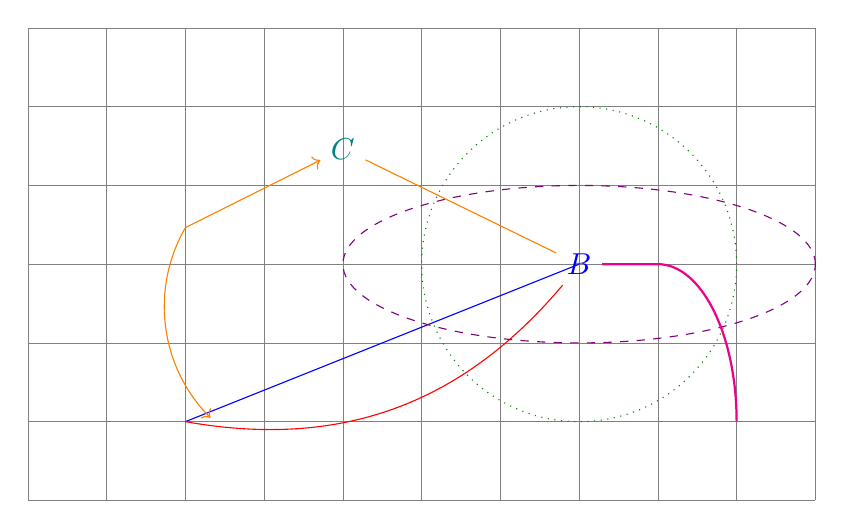
\begin{tikzpicture}
\foreach \x in {0,1,...,10} {\draw[gray,very thin] (\x,0)--++(0,6);}
\foreach \y in {0,1,...,6} {\draw[gray,very thin] (0,\y)--++(10,0);}
\coordinate(A)at(2,1);
\draw[blue] (A)--++(5,2)node(B){$B$};
\draw[red] (A)to[bend right=30](B);
\draw[Green,dotted](B)circle(2);
\draw[violet,dashed](B)ellipse(3cm and 1cm);
\node[teal](C)at($(A)+(60:4)$){$C$};
\draw[orange,<->](B)--(C)--++(-2,-1)arc(150:225:2);
\draw[magenta,thick](B)--++(1,0)arc(90:0:1cm and 2cm);
\end{tikzpicture}
\end{figure}
\fi

\newpage
\section{Introduzione al pacchetto \liLaTeXtikz}
Il pacchetto \liLaTeXtikz\ estende il pacchetto \ttt{tikz} con una serie di comandi. Questi sono utili soprattutto per produrre disegni di geometria euclidea ed analitica, ma in piccola parte anche per produrre immagini utili nell'ambito della fisica.

Molte delle funzioni implementate si appoggiano al pacchetto \ttt{tkz-euclide}, che contiene numerosi comandi per la produzione di immagini utili per la geometria euclidea. Il pacchetto \ttt{tkz-euclide} in realtà è molto più ampio del pacchetto \liLaTeXtikz, e contiene numerose funzioni che non sono direttamente implementate in \liLaTeXtikz. Tuttavia la sintassi usata in \ttt{tkz-euclide} a mio avviso risulta piuttosto controintuitiva e poco concisa, il che rende \liLaTeXtikz\ preferibile per la produzione di immagini semplici. \ttt{tkz-euclide} risulta invece preferibile per produrre immagini particolarmente elaborate.

\section{L'ambiente \ttt{immagine}}
In \ttt{tikz} le immagini vengono normalmente racchiuse nell'ambiente \ttt{tikzpicture}. Questo vuol dire che un'immagine viene racchiusa fra una stringa \ttt{\bs begin\{tikzpicture\}[\opzioni]} e una stringa \ttt{\bs end\{tikzpicture\}}

In \liLaTeXtikz\ utilizziamo invece l'ambiente \ttt{immagine}. Un'immagine viene quindi racchiusa fra una stringa \ttt{\bs begin\{immagine\}[\opzioni]} e una stringa \ttt{\bs end\{immagine\}}. La sintassi è quindi

\comando{\bs begin\{immagine\}[\opzioni] \textcolor{brown}{body} \bs end\{immagine\}}

Le opzioni possono specificare il colore o la scala. Ad esempio, scrivendo

\ttt{\bs begin\{immagine\}[\blue{red,scale=0.5}] \textcolor{brown}{body} \bs end\{immagine\}}

produrremo un'immagine in cui il colore di default è il rosso (anziché il nero) e in cui tutte le misure sono dimezzate.

\subsection{Gli ambienti \ttt{immaginecap} e \ttt{immaginecap*}}
Gli ambienti \ttt{immaginecap} e \ttt{immaginecap*} funzionano in modo analogo all'ambiente \ttt{immagine} e vanno usati quando intendiamo inserire una caption all'immagine. La sintassi (analoga per i due ambienti) è

\comando{\bs begin\{immaginecap\}[\opzioni]\{\blue{caption}\} \textcolor{brown}{body} \bs end\{immaginecap\}}

La differenza è che \ttt{immaginecap} numera le caption, mentre \ttt{immaginecap*} non include la numerazione delle caption.

\section{L'ambiente \ttt{rotazione}}
Un altro importante ambiente è l'ambiente \ttt{rotazione}, definito tramite la seguente sintassi

\comando{\bs begin\{rotazione\}[centro := \keyval{$(0,0)$}]\{angolo\} \textcolor{brown}{body} \bs end\{rotazione\}}

L'\ttt{angolo} indica l'angolo di rotazione (in gradi in senso antiorario), mentre il \ttt{centro} indica il centro di rotazione (se non specificato si assume una rotazione attorno all'origine).

\textbf{Attenzione!} se all'interno del \textcolor{brown}{body} si inserisce una coordinata come $(2,1)$ questa verrà regolarmente ruotata. Se però si crea un punto $A=(2,1)$ fuori dall'ambiente \ttt{rotazione} e si usa $A$ dentro all'ambiente rotazione questo non verrà ruotato. Il comportamento (controintuitivo) è illustrato nel seguente esempio:

\begin{Verbatim}[frame=single]
\node(O)at(2,0){$O$};
\coordinate(A)at(3,0.5);
\begin{rotazione}[O]{+90}
  \node[red](Al)at(A){$A$};
  \node[blue](Bl)at(3,0.5){$B$};
\end{rotazione}
\end{Verbatim}
\vspace*{-4mm}

\ifnum\showimmagini=1
\begin{immagine}
\node(O)at(2,0){$O$};
\coordinate(A)at(3,0.5);
\begin{rotazione}[O]{+90}
  \node[red](Al)at(A){$A$};
  \node[blue](Bl)at(3,0.5){$B$};
\end{rotazione}
\end{immagine}
\fi

\newpage
\section{L'uso delle keys in \liLaTeXtikz}
Il pacchetto \liLaTeXtikz\ contiene diversi comandi. Alcuni di questi comandi hanno delle \opzioni\ come argomenti opzionali. Questi tendenzialmente sono gli stessi previsti per \ttt{\bs draw} e illustrati nella sezione \ref{opzsec}.

Altri comandi come argomento opzionale accettano invece delle \keys.

Per le keys è prevista una sintassi un po' più articolata. Ad esempio, per disegnare un segmento con \ttt{\bs draw} (che usa delle \opzioni) scriviamo \ttt{\bs draw[red]...;}. Per disegnare un segmento rosso col comando \ttt{\bs segmento} (che usa delle \keys) scriviamo invece \ttt{\bs segmento[col=red]...;}. Così facendo si sta dando il valore \keyval{red} alla chiave chiamata \key{col} (che nel caso di \ttt{\bs comando} rappresenta il colore del segmento).

\subsection{Chiavi comuni e loro valori predefiniti}\label{keysec}
Questo è un elenco delle \keys\ più comuni e dei valori di default che contengono di solito:
\begin{itemize}
\item \key{col} indica il colore dell'oggetto da disegnare, e di un suo eventuale label. Se non specificato è in genere inizializzato come il colore dell'immagine (generalmente \keyval{black}).
\item \key{col draw} in alcuni casi specifica il colore delle linee. Se non specificato copia \key{col}.
\item \key{col lbl} e il suo sinonimo \key{lbl col} indicano il colore del label. Se non specificato copia il valore in \key{col}.
\item \key{col fill} il colore del filling. Se non specificato copia il valore in \key{col}.
\item \key{opacity} se specificato \key{col fill} (se lasciato vuoto) copia \key{col}!\key{opacity} anziché \key{col}.
\item \ttt{\key{fill} := \keyval{false}} può essere settato a \keyval{true} se vogliamo colorare l'interno della figura. Diventa automaticamente \keyval{true} se specifichiamo \key{col fill}.
\item \key{width} lo spessore della linea. Se non specificato la linea viene disegnata di spessore normale (ovvero \keyval{semithick}). Accetta valori come \keyval{thin} e \keyval{thick}, ma anche \keyval{very thick} e \keyval{ultra thick} (o \keyval{very thin} e \keyval{ultra thin}).
\item \key{pattern} è il pattern della linea. Il valore di default è la linea continua (ovvero \keyval{solid}) ma può assumere anche valori come \keyval{dashed} o \keyval{dotted}.
\item \key{arrow} permette di specificare se vogliamo che la linea si concluda con una freccia. In genere il default è vuoto, ma si possono specificare frecce come \keyval{<-}, \keyval{->}, \keyval{<->}, \keyval{|<->|} o \keyval{|->}.
\item \key{lbl} il nome da dare al label. Se non specificato in genere non viene creato un label.
\item \key{lbl size} vuoto di default. Se specificato (con valori come \keyval{large}, \keyval{small} o \keyval{tiny}) cambia la dimensione del label.
\item \ttt{\key{lbl dist} := \keyval{0.3}} la distanza del label dal nodo.
\item \key{lbl name} il nome da dare alla posizione del label. Il valore di default cambia di funzione in funzione.
\item \ttt{\key{mark} := \keyval{none}} il segno da mettere su un segmento / angolo / arco. Le opzioni sono \keyval{none} (se non vogliamo nessun segno) oppure: \keyval{s}, \keyval{z}, \keyval{x}, \keyval{o}, \keyval{oo}, \keyval{|}, \keyval{||}, \keyval{|||} (lista esaustiva).
\item \ttt{\key{mark size} := \keyval{0.2}} la dimensione del segno definito con \key{mark}.
\item \key{col mark} il colore del segno (se non specificato diventa \keyval{black}).
\item \ttt{\key{side} := \keyval{->}} può assumere anche il valore \keyval{<-} e indica come deve essere orientata l'immagine (utile per alcune immagini ``complesse'').
\end{itemize}

\subsection{Le keys opzionali}
In alcuni casi è possibile definire delle \keys\ opzionali. Un esempio può essere la chiave \keyop{mirror} per \ttt{\bs auto} (e per molte altre funzioni simili).

Per queste keys non serve assegnare un valore esplicitamente.

Le più comuni sono:
\begin{itemize}[nolistsep]
\item \keyop{mirror}, che, se specificata, riflette l'immagine.
\item \keyop{fill}, che, se specificata, riempie l'interno dell'immagine. Alcuni comandi usano invece \keyop{no fill}.
\item \keyop{no label}, che se specificata rimuove i label dell'immagine.
\end{itemize}

Vediamo un semplice esempio:

\begin{Verbatim}[frame=single]
\auto[col=blue]{0,0};
\auto[col=red,mirror]{4,0};
\circCR[col=Green]{8,1}{1};
\circCR[col=orange,fill]{11,1}{1};
\end{Verbatim}
\vspace*{-4mm}

\ifnum\showslowimmagini=1
\begin{immagine}[scale=0.5]
\auto[col=blue]{0,0};
\auto[col=red,mirror]{4,0};
\circCR[col=Green]{8,1}{1};
\circCR[col=orange,fill]{11,1}{1};
\end{immagine}
\fi

Per vedere come definire una key opzionale si rimanda all'esempio della key opzionale \keyop{mirror} definita nel comando \ttt{\bs auto}.

\subsection{Il key-manager in \liLaTeXtikz}
Il key-manager di \liLaTeXtikz\ è una parte interna a \liLaTeXtikz\ di cui l'utente normale non deve preoccuparsi, ma che risulta importante per chi intende modificare/estendere il pacchetto.

Contiene alcune funzioni importanti che vengono elencate qui di seguito:

\comandons{\bs ifkeyempty\{\blue{KEY}\}\{\blue{TRUE}\}\{\blue{FALSE}\};}
controlla se la key \blue{KEY} è vuota. Se è vuota esegue il comando \blue{TRUE}, altrimenti esegue il comando \blue{FALSE}.

\comandons{\bs ifkeyequal\{\blue{KEY}\}\{\blue{str}\}\{\blue{TRUE}\}\{\blue{FALSE}\};}
controlla se la key \blue{KEY} è uguale alla stringa \blue{str}. Se è uguale esegue il comando \blue{TRUE}, altrimenti esegue il comando \blue{FALSE}.

Il comando

\comandons{\bs setkeyvalue\{\blue{KEY}\}\{\blue{val}\};}
assegna il valore \blue{val} alla key \blue{KEY}, mentre il comando

\comandons{\bs copykeyvalue\{\blue{KEYto}\}\{\blue{KEYfr}\};}
copia il valore della key \blue{KEYfr} nella key \blue{KEYto}.

I comandi \ttt{\bs setkeyvalueifempty\{\blue{KEY}\}\{\blue{val}\};} e \ttt{\bs copykeyvalueifempty\{\blue{KEYto}\}\{\blue{KEYfr}\};} funzionano in modi analoghi, ma si attivano solo se la key da sovrascrivere (quella nel primo input) è vuota.

Ci sono infine i comandi

\comando{\bs setkeyvaluesifempty\{\blue{KEY1}\}\{\blue{val1}\}\{\blue{KEY2}\}\{\blue{val2}\}\{\blue{KEY3}\}\{\blue{val3}\}\dots;}
\comandons{\bs copykeyvaluesifempty\{\blue{KEYto1}\}\{\blue{KEYfr1}\}\{\blue{KEYto2}\}\{\blue{KEYfr2}\}\{\blue{KEYto3}\}\{\blue{KEYfr3}\}\dots;}
che ripetono rispettivamente \ttt{\bs setkeyvalueifempty} e \ttt{\bs copykeyvalueifempty} per tutte le coppie specificate.

\subsection{Le funzioni PRIV}\label{PRIVsec}
All'interno del pacchetto \liLaTeXtikz\ sono presenti alcune funzioni il cui nome inizia con la stringa \ttt{PRIV}. Queste sono funzioni \textit{private} e non devono essere utilizzate dall'utente. Il loro scopo è di essere utilizzate internamente da altre funzioni all'interno del pacchetto \liLaTeXtikz.

Le \keys\ di queste funzioni hanno dei nomi un po' particolari (che iniziano, a loro volta, con la stringa \ttt{PRIV}), in modo da non poter essere sovrascritte accidentalmente dall'utente quando vengono specificati i valori di \keys\ di funzioni pubbliche (quelle non private).

L'utente medio non deve ignorare queste funzioni, che risultano invece molto importanti per chi desidera modificare/estendere il pacchetto \liLaTeXtikz.

\newpage
\section{La funzione \ttt{\bs griglia}}
A volte siamo interessati a disegnare una griglia (una parte di foglio a quadretti). Per farlo utilizziamo il comando

\comandons{\bs griglia[\keys]\{\blue{Ovest}\}\{\blue{Est}\}\{\blue{Sud}\}\{\blue{Nord}\};}
Dove gli argomenti \ttt{Ovest}, \ttt{Est}, \ttt{Sud} e \ttt{Nord} indicano i confini della griglia.

Se dobbiamo porre \ttt{Est} e \ttt{Sud} entrambi a zero, possiamo usare anche la seguente sintassi equivalente:

\comando{\bs grigliaO[\keys]\{\blue{Est}\}\{\blue{Nord}\};}

Le \keys\ sono:
\begin{itemize}[nolistsep]
\item \ttt{\key{col} := \keyval{gray!50}}, \ttt{\key{width} := \keyval{thin}}, \key{pattern} come spiegate nella sezione \ref{keysec};
\item \key{col fill}. Se specificato l'interno delle griglia viene colorato col colore specificato;
\item \ttt{\key{s} = \key{step} := \keyval{1}} specificano la distanza fra due linee. Volendo possono essere definite separatamente per le due direzioni come \ttt{\key{s x} = \key{step x}} e \ttt{\key{s y} = \key{step y}}.
\end{itemize}

Vediamo un esempio:

\begin{Verbatim}[frame=single]
\grigliaO[s y=0.5,col=pink]{3}{2};
\griglia[s=0.4]{4}{7}{0}{1};
\griglia[col fill=yellow!30]{8}{10.5}{0}{2.5};
\end{Verbatim}
\vspace*{-4mm}

\ifnum\showimmagini=1
\begin{immagine}
\grigliaO[s y=0.5,col=pink]{3}{2};
\griglia[s=0.4]{4}{7}{0}{1};
\griglia[col fill=yellow!30]{8}{10.5}{0}{2.5};
\end{immagine}
\fi

\subsection{La carta millimetrata}
In fisica siamo spesso interessati a riprodurre parti di carta millimetrata. Ciò può essere fatto utilizzando il comando

\comandons{\bs cartamillimetrata[\keys]\{\blue{Ovest}\}\{\blue{Est}\}\{\blue{Sud}\}\{\blue{Nord}\};}
dove \ttt{Ovest}, \ttt{Est}, \ttt{Sud} e \ttt{Nord} hanno gli stessi significati appena spiegati per la funzione \ttt{\bs griglia}.

In questo caso le \keys sono:
\begin{itemize}[nolistsep]
\item \ttt{\key{col1} := \keyval{pink!50}}, \ttt{\key{width1} := \keyval{ultra thin}}, \key{pattern1} e \ttt{\key{s1} = \key{step1} := \keyval{0.1}} analoghi ai loro analoghi in \ttt{\bs griglia} (per il tratto più sottile).
\item \ttt{\key{col2} := \keyval{gray!70}}, \key{width2} := \keyval{thin}, \key{pattern2} e \ttt{\key{s2} = \key{step2} := \keyval{0.5}} analoghi per il tratto più spesso.
\end{itemize}

C'è anche la possibilità di creare un'intera pagina di carta millimetrata usando il comando

\comandons{\bs cartamillimetratapagina[\keys];}
con le stesse \keys.

\textbf{Attenzione!} Il comando \ttt{\bs cartamillimetratapagina} funziona solo se \ttt{\bs TipoDoc = \keyval{immagine}}. Per inserire una pagina di carta millimetrata all'interno di un altro documento conviene quindi generare la pagina di carta millimetrata in un altro documento, e poi includere la pagina in questione all'interno del documento reale usando un \ttt{\bs includepdf}.

\newpage
\section{Gli assi cartesiani}
Spesso è utile disegnare sistemi di riferimento cartesiani. In questa sezione del manuale vedremo alcuni comandi utili per disegnare assi cartesiani di vari tipi.

\subsection{Gli assi del piano cartesiano}
Se disegniamo un piano cartesiano siamo interessati anche a disegnare gli assi cartesiani.

Gli assi cartesiani possono essere disegnati uno per volta usando i comandi

\comando{\bs assex[\keys]\{\blue{Ovest}\}\{\blue{Est}\};}\\
\comando{\bs assey[\keys]\{\blue{Sud}\}\{\blue{Nord}\};}

con le \keys:
\begin{itemize}[nolistsep]
\item \key{col}, \key{width}, \key{pattern}, \ttt{\key{arrow} := \keyval{->}}, \key{lbl}, \key{lbl name}, \key{lbl size}, \key{lbl dist}, \ttt{\key{lbl col} = \key{col lbl}} coi significati della sezione \ref{keysec}.
\item \ttt{\key{y} := \keyval{0}} (solo per \ttt{\bs assex}) specifica la coordinata $y$ dell'asse delle ascisse. Analogamente \ttt{\key{x} := \keyval{0}} (solo per \ttt{\bs assey}) specifica la coordinata $x$ dell'asse delle ordinate.
\item \ttt{\key{ang shift} := \keyval{0}} una rotazione extra per il label (oltre a quella prevista dalla posizione iniziale).
\item L'opzione \keyop{mirror lbl}, se specificata, ruota il label di $180^\circ$.
\end{itemize}

Volendo è anche possibile definire i due assi cartesiani insieme col comando

\comando{\bs assexy[\keys]\{\blue{Ovest}\}\{\blue{Est}\}\{\blue{Sud}\}\{\blue{Nord}\};}

o equivalentemente (se vogliamo traslare il centro) come

\comando{\bs assexyO[\keys]\{centro\}\{\blue{Ovest}\}\{\blue{Est}\}\{\blue{Sud}\}\{\blue{Nord}\};}

Entrambi i comandi hanno le seguenti \keys:
\begin{itemize}[nolistsep]
\item \key{col}, \key{width}, \key{pattern}, \ttt{\key{arrow} := \keyval{->}}, \ttt{\key{lbl dist} := \keyval{0.3}}, \ttt{\key{lbl col} = \key{col lbl}} coi significati della sezione \ref{keysec}.
\item \ttt{\key{lbl x} := \keyval{\$x\$}} e \ttt{\key{lbl y} := \keyval{\$y\$}} sono i due label.
\item \key{lbl x name} e \key{lbl y name} sovrascrivono sono i nomi dei due label.
\item \ttt{\key{x} := \keyval{0}} e \ttt{\key{y} := \keyval{0}} (solo per \ttt{\bs assexy}) specifica le coordinate del centro del sistema di riferimento.
\end{itemize}

\subsubsection{Le barre per gli assi cartesiani}
Spesso vogliamo aggiungere delle barre per indicare alcuni valori numerici sugli assi cartesiani. Questi in genere vengono usati all'interno di un loop \ttt{\bs foreach}. Questo può essere fatto coi comandi:

\comando{\bs assexbar[\keys]\{\blue{\bs x}\}\{\blue{lbl}\};}\\
\comando{\bs asseybar[\keys]\{\blue{\bs y}\}\{\blue{lbl}\};}

Le coordinate \ttt{\bs x} e \ttt{\bs y} nei due comandi indicano le posizioni della tacca, mentre \ttt{lbl} indica il label che vogliamo scrivere. Le \keys\ sono:
\begin{itemize}[nolistsep]
\item \key{col}, \ttt{\key{width} := \keyval{very thin}}, \key{pattern}, \key{arrow}, \ttt{\key{lbl col} = \key{col lbl}} coi significati della sezione \ref{keysec}.
\item \ttt{\key{l} = \key{length} := \keyval{0.2}} la lunghezza della barretta.
\item \ttt{\key{y} := \keyval{0}} (solo per \ttt{\bs assexbar}) e \ttt{\key{x} := \keyval{0}} (solo per \ttt{\bs asseybar}) è l'altra coordinata del centro della barretta.
\item L'opzione \keyop{\bs mirror}, se specificata, pone i label verso l'alto (nel caso di \ttt{\bs assexbar}) o verso destra (nel caso di \ttt{\bs asseybar}).
\end{itemize}

Il seguente esempio illustra come utilizzare il sistema cartesiano in un caso semplice.

\begin{Verbatim}[frame=single]
\griglia[s=0.5]{-1}{10}{-1}{5};
\assixy{-1}{9.7}{-1}{4.7};
\foreach \x in {1,2,...,9} \assexbar{\x}{$\x$};
\foreach \y in {-1,1,2,...,8} \asseybar[mirror]{0.5*\y}{$\y$};
\end{Verbatim}
\vspace*{-4mm}

\ifnum\showimmagini=1
\begin{immagine}
\griglia[s=0.5]{-1}{10}{-1}{5};
\assixy{-1}{9.7}{-1}{4.7};
\foreach \x in {1,2,...,9} \assexbar{\x}{$\x$};
\foreach \y in {-1,1,2,...,8} \asseybar[mirror]{0.5*\y}{$\y$};
\end{immagine}
\fi

\subsection{Sistemi di riferimento in fisica col comando \ttt{\bs sistrif}}
Il comando \ttt{\bs sistrif} consente di inserire un sistema di riferimento (eventualmente ruotato) all'interno di un'immagine di fisica. Lo si usa con la sintassi seguente:

\comandons{\bs sistrif[\keys]\{\blue{centro}\}\{\blue{angolo}\};}
dove \ttt{centro} indica il centro del sistema di riferimento (dove vogliamo disegnare l'origine), mentre \ttt{angolo} indica l'angolo di inclinazione dell'asse $x$. Le \keys\ sono:
\begin{itemize}[nolistsep]
\item \ttt{\key{col} := \keyval{magenta}}, \ttt{\key{lbl col} = \key{col lbl}}, \key{width}, \key{pattern}, \ttt{\key{arrow} := \keyval{->}}, \ttt{\key{lbl dist} := \keyval{0.3}} come spiegate nella sezione \ref{keysec}. Si riferiscono a entrambi gli assi cartesiani.
\item \ttt{\key{front} := \keyval{2}} e \ttt{\key{back} := \keyval{0.3}} indicano le lunghezze dei due assi cartesiani in avanti (per valori positivi) e indietro (per valori negativi). Possono essere sovrascritti separatamente per i due assi con le \keys\ \key{front x}, \key{front y}, \key{back x} e \key{back y}.
\item \ttt{\key{lbl x} := \keyval{\$x\$}} e \ttt{\key{lbl y} := \keyval{\$y\$}} sono i label per i due assi cartesiani. Se si vuole togliere un label scrivere, ad esempio, \ttt{\key{lbl x}=}.
\item L'opzione \keyop{no label}, se specificata, rimuove i label.
\item L'opzione \keyop{filp} può essere specificata se vogliamo che l'asse $y$ si trovi ruotato di $90^\circ$ in senso \textit{orario} (anziché \textit{antiorario}) rispetto all'asse $y$.
\end{itemize}

Vediamo un semplice esempio:

\begin{Verbatim}[frame=single]
\sistrif[no label]{0,0}{0};
\sistrif[col=teal,lbl x=$t$]{4,0}{30};
\sistrif[col=gray!70,lbl x=$\ra$,mirror]{8,0}{15};
\end{Verbatim}
\vspace*{-4mm}

\ifnum\showimmagini=1
\begin{immagine}
\sistrif[no label]{0,0}{0};
\sistrif[col=teal,lbl x=$t$]{4,0}{30};
\sistrif[col=gray!70,lbl x=$\ra$,mirror]{8,0}{15};
\end{immagine}
\fi

\newpage
\section{I punti con \ttt{\bs punto}}
La funzione principale di \liLaTeXtikz\ è la funzione che crea dei punti usando la sintassi

\comando{\bs punto[\keys]\{\blue{coordinate}\};}

con le \keys:
\begin{itemize}[nolistsep]
\item \key{col}, \ttt{\key{lbl col} = \key{col lbl}}, \key{lbl}, \key{lbl name}, \key{lbl size}, \ttt{\key{lbl dist} := \keyval{0.3}} come spiegate nella sezione \ref{keysec}.
\item \ttt{\key{lbl ang} := \keyval{-90}} l'angolo a cui si trova il label (se specificato).
\item \ttt{\key{name} := \keyval{puntoNome}} il nome da dare al punto (non al label).
\item \ttt{\key{size} := \keyval{1.5}} la dimensione del punto (in \ttt{pt}).
\item \ttt{\key{shape} := \keyval{circle}} la forma del punto. Può essere posto a \keyval{rectangle}.
\end{itemize}

\subsection{I punti con sintassi concisa come \ttt{\bs pnt}, \ttt{\bs pntlbl} e \ttt{\bs pntl}}

Spesso vogliamo specificare solo alcune delle keys di \ttt{\bs punto}. Per farlo ci sono i seguenti comandi più concisi, che internamente richiamano \ttt{\bs punto}. Vogliamo invece chiamare esplicitamente \ttt{\bs punto} se vogliamo personalizzare altri parametri:

\comandons{\bs pnt[\textcolor{gray}{col}]\{\blue{name}\}\{\blue{coordinate}\};}
utile se non vogliamo inserire un label.

Se invece vogliamo un label, la versione più generale è

\comando{\bs pntlbl[\textcolor{gray}{col}]\{\blue{name}\}\{\blue{lbl}\}\{\blue{lbl ang}\}\{\blue{coordinate}\};}

Ci sono infine versioni di \ttt{\bs pntlbl} ancora più concise, in cui il label coincide col nome (circa):

\comando{\bs pntl[\textcolor{gray}{col}]\{\blue{name}\}\{\blue{lbl ang}\}\{\blue{coordinate}\}; \hspace*{1cm}\textcolor{gray}{\% \key{lbl} := \$\blue{name}\$}}

\comando{\bs pntlp[\textcolor{gray}{col}]\{\blue{nome}\}\{\blue{lbl ang}\}\{\blue{coordinate}\}; \hspace*{1cm}\textcolor{gray}{\% \key{name} := \blue{nome}p, \key{lbl} := \$\blue{nome}'\$}}

\comando{\bs pntls[\textcolor{gray}{col}]\{\blue{nome}\}\{\blue{lbl ang}\}\{\blue{coordinate}\}; \hspace*{1cm}\textcolor{gray}{\% \key{name} := \blue{nome}s, \key{lbl} := \$\blue{nome}''\$}}

Vediamo un semplice esempio illustrativo.

\begin{Verbatim}[frame=single]
\grigliaO{9}{2};
\punto[shape=rectangle,size=2.5]{1,1};
\pnt[orange]{T}{2,1};
\pntlbl[violet]{A}{$A$}{45}{4,1};
\draw[->,magenta] (T)--(A);
\pntl[blue]{P}{-90}{6,1};
\pntlp[red]{P}{-90}{7,1}; % il punto si chiama Pp
\pntls[Green]{P}{0}{8,1}; % il punto si chiama Ps
\draw[->,teal] (Pp) to[bend left=90] (Ps);
\end{Verbatim}
\vspace*{-4mm}

\ifnum\showimmagini=1
\begin{immagine}
\grigliaO{9}{2};
\punto[shape=rectangle,size=2.5]{1,1};
\pnt[orange]{T}{2,1};
\pntlbl[violet]{A}{$A$}{45}{4,1};
\draw[->,magenta] (T)--(A);
\pntl[blue]{P}{-90}{6,1};
\pntlp[red]{P}{-90}{7,1}; % il punto si chiama Pp
\pntls[Green]{P}{0}{8,1}; % il punto si chiama Ps
\draw[->,teal] (Pp) to[bend left=90] (Ps);
\end{immagine}
\fi

\textbf{Attenzione!} I punti definiti con \ttt{\bs punto} e i suoi derivati non sono compatibili con la chiave \key{fill} di \ttt{\bs draw}. Se vogliamo usare la chiave \key{fill} serve quindi definire i punti tramite \ttt{\bs coordinate}, e poi ripassarli in un secondo momento (dopo aver usato la chiave \key{fill} dove ci serve).

\newpage
\section{L'aggiunta dei label con \ttt{\bs stylelbl}}
Aggiungere label può essere molto scomodo. Soprattutto se vogliamo scrivere il label usando un ambiente matematico (\ttt{\bs mathrm}, \ttt{\bs mathbf} o \ttt{\bs mathcal}). Per fare ciò, nel pacchetto \liLaTeXtikz\ è definito un comando specifico:

\comandons{\bs stylelbl[\keys]\{\blue{posizione}\};}
dove \ttt{coord} è la posizione del punto dove creare il label. Le \keys\ sono:
\begin{itemize}[nolistsep]
\item \key{lbl}, \key{lbl size}, \ttt{\key{lbl name} := \keyval{scriptlblName}}, \ttt{\key{col lbl} = \key{lbl col} = \key{col}} come spiegate nella sezione \ref{keysec}.
\end{itemize}

\section{Intersezioni con \ttt{\bs intrette} e \ttt{\bs intpaths}}\label{intersezionisec}
Il comando \ttt{\bs interette} ci permette di creare un punto $P$ come l'intersezione fra due rette $AB$ e $CD$. La sintassi è

\comando{\bs intrette\{\Green{P}\}\{\blue{A}\}\{\blue{B}\}\{\blue{C}\}\{\blue{D}\};}

Possiamo anche trovare un punto $P$ di intersezione fra due paths chiamati \ttt{path1} e \ttt{path2} usando la sintassi

\comando{\bs intpaths\{\Green{P}\}\{\blue{path1}\}\{\blue{path2}\};}

I due comandi sono illustrati nel seguente esempio:

\begin{Verbatim}[frame=single]
\grigliaO{10}{3};
\draw(1,0)--(7,3) (0,2)--++(10,0);
\intrette{P}{1,0}{3,1}{0,2}{1,2};
\pntl[blue]{P}{90}{P};
\draw[Green,dashed,name path=circ](P)circle(1);
\draw[name path=line,->](P)--++(-45:2);
\intpaths{Q}{circ}{line};
\punto[col=red]{Q};
\end{Verbatim}
\vspace*{-4mm}

\ifnum\showimmagini=1
\begin{immagine}
\grigliaO{10}{3};
\draw(1,0)--(7,3) (0,2)--++(10,0);
\intrette{P}{1,0}{3,1}{0,2}{1,2};
\pntl[blue]{P}{90}{P};
\draw[Green,dashed,name path=circ](P)circle(1);
\draw[name path=line,->](P)--++(-45:2);
\intpaths{Q}{circ}{line};
\punto[col=red]{Q};
\end{immagine}
\fi

\newpage\section{Funzioni con punti in input e un numero come output}
All'interno del pacchetto \liLaTeXtikz\ sono presenti alcune funzioni che restituiscono un numero in output (prendendo dei punti come input). Queste sono le funzioni principali:

\comandons{\bs distanza\{\Green{\bs d}\}\{\blue{A}\}\{\blue{B}\};}
scrive in \ttt{\bs d} la distanza fra $A$ e $B$.

\comandons{\bs angolopolare\{\Green{\bs and}\}\{\blue{P}\}\{\blue{O}\};}
scrive in \ttt{\bs ang} l'angolo del vettore $\vc{OP}$ (in gradi).

Vediamo un semplice esempio:

\begin{Verbatim}[frame=single]
\pntl{A}{180}{0,0};
\pntl{B}{35}{35:1.5};
\distanza{\r}{A}{B};
\angolopolare{\a}{B}{A};
\draw[red,thin,dashed] (A) circle (\r);
\pntlp[blue]{B}{-35}{-\a:\r};
\end{Verbatim}
\vspace*{-4mm}

\ifnum\showimmagini=1
\begin{immagine}
\pntl{A}{180}{0,0};
\pntl{B}{35}{35:1.5};
\distanza{\r}{A}{B};
\angolopolare{\a}{B}{A};
\draw[red,thin,dashed] (A) circle (\r);
\pntlp[blue]{B}{-35}{-\a:\r};
\end{immagine}
\fi

\section{Manipolazione di coordinate}
Il pacchetto \liLaTeXtikz\ contiene diverse funzioni che ci permettono di manipolare le coordinate.

Le principali sono descritte in questa sezione:

\comandons{\bs verso[\teal{L} := \keyval{1}]\{\Green{P}\}\{\blue{A}\}\{\blue{B}\};}
crea un punto $P$ sulla semiretta $AB$ (a distanza \ttt{L} da $A$).

\comandons{\bs allont[\teal{L} := \keyval{1}]\{\Green{P}\}\{\blue{A}\}\{\blue{B}\};}
crea un punto $P$ sulla semiretta $BA$ (a distanza \ttt{L} da $A$).

\comandons{\bs parallelo[\teal{L} := \keyval{1}]\{\Green{P}\}\{\blue{S}\}\{\blue{A}\}\{\blue{B}\};}
crea un punto $P$, ottenuto traslando $S$ per una lunghezza $L$ nel verso nel vettore $\vc{AB}$.

\comandons{\bs perpendicolare[\teal{L} := \keyval{1}]\{\Green{P}\}\{\blue{S}\}\{\blue{A}\}\{\blue{B}\};}
crea un punto $P$, ottenuto traslando $S$ per una lunghezza $L$ nel verso perpendicolare a $\vc{AB}$ (si suppone $SAB$ in senso antiorario).

\comandons{\bs medio[\teal{k} := \keyval{0.5}]\{\Green{M}\}\{\blue{A}\}\{\blue{B}\};}
definisce $M$ come il punto $(1-k)*A+k*B$. Nel caso speciale di $k=0.5$, $M$ è il punto medio del segmento $AB$. Quindi se $k=0$ risulta $M:=A$, mentre se $k=1$ risulta $M:=B$.

\comandons{\bs opposto\{\Green{P'}\}\{\blue{P}\}\{\blue{O}\};}
definisce il punto $P'$ come l'opposto di $P$ rispetto ad $O$ (quindi $O$ risulterà essere il punto medio di $PP'$).

\comandons{\bs simmetrico\{\Green{P'}\}\{\blue{P}\}\{\blue{A}\}\{\blue{B}\};}
definisce il punto $P'$ come il simmetrico di $P$ rispetto alla retta $AB$.

\comandons{\bs proj\{\Green{H}\}\{\blue{P}\}\{\blue{A}\}\{\blue{B}\};}
definisce il punto $H$ come la proiezione ortogonale di $P$ sulla retta $AB$.

\comandons{\bs sumvett\{\Green{C}\}\{\blue{A}\}\{\blue{B}\}\{\blue{D}\};}
definisce il punto $C$ in modo che $\vc{AC}=\vc{AB}+\vc{AD}$. Questo vuol dire in particolare che $C$ sarà definito in modo che il quadrilatero $ABCD$ sia un parallelogramma.

\comandons{\bs ruotapunto\{\Green{R}\}\{\blue{P}\}\{\blue{O}\}\{\blue{a}\};}
definisce il punto $R$ ottenuto ruotando $P$ in senso antiorario di un angolo \ttt{a} (con centro di rotazione in $O$).

\comandons{\bs ruotapuntoN[\teal{N} := \keyval{1}]\{\Green{R}\}\{\blue{P}\}\{\blue{O}\}\{\blue{a}\};}
analogo a \ttt{\bs ruotapunto} ma normalizza il vettore $\vc{OR}$ in modo che misuri \ttt{L}.

\comandons{\bs triangoloequilatero\{\Green{C}\}\{\blue{A}\}\{\blue{B}\};}
crea un punto $C$ in modo che il triangolo $ABC$ sia equilatero (con vertici in senso antiorario).

Vediamo un esempio in cui sono illustrate le funzioni di questa sezione.

\begin{Verbatim}[frame=single]
\grigliaO{12}{5};
\pntl{A}{-90}{3,1};
\pntl{B}{90}{5,3};
\pntl{C}{135}{2,2};
\verso{D}{A}{B};
\pntl[violet]{D}{0}{D};
\allont[2]{E}{B}{C};
\pntl[red]{E}{135}{E};
\parallelo[2]{F}{D}{B}{E};
\pntl[blue]{F}{-45}{F};
\perpendicolare{G}{D}{B}{E};
\pntl[teal]{G}{-45}{G};
\medio[0.7]{M}{B}{C};
\pntl[orange]{M}{90}{M};
\opposto{Mp}{M}{C};
\pntlp[green]{M}{90}{Mp};
\simmetrico{Bp}{B}{D}{F};
\pntlp[green]{B}{-30}{Bp};
\proj{H}{B}{D}{F};
\pntl[magenta]{H}{-120}{H};
\sumvett{V}{B}{E}{F};
\pntl[cyan]{V}{-90}{V};
\ruotapunto{R}{E}{V}{-150};
\pntl[pink]{R}{-90}{R};
\ruotapuntoN[3]{Rp}{E}{V}{-150};
\pntlp[pink]{R}{-90}{Rp};
\triangoloequilatero{T}{R}{Rp};
\pntl[brown]{T}{90}{T};
\draw[gray] (Mp)--(C)--(M)--(B)--(E)--(V)--(F)--(H)--(D)--(G);
\draw[gray] (A)--(D)--(B) (F)--(B)--(H)--(Bp) (V)--(R)--(Rp)--(T)--(R);
\end{Verbatim}
\vspace*{-4mm}

\ifnum\showimmagini=1
\begin{immagine}
\grigliaO{12}{5};
\pntl{A}{-90}{3,1};
\pntl{B}{90}{5,3};
\pntl{C}{135}{2,2};
\verso{D}{A}{B};
\pntl[violet]{D}{0}{D};
\allont[2]{E}{B}{C};
\pntl[red]{E}{135}{E};
\parallelo[2]{F}{D}{B}{E};
\pntl[blue]{F}{-45}{F};
\perpendicolare{G}{D}{B}{E};
\pntl[teal]{G}{-45}{G};
\medio[0.7]{M}{B}{C};
\pntl[orange]{M}{90}{M};
\opposto{Mp}{M}{C};
\pntlp[green]{M}{90}{Mp};
\simmetrico{Bp}{B}{D}{F};
\pntlp[green]{B}{-30}{Bp};
\proj{H}{B}{D}{F};
\pntl[magenta]{H}{-120}{H};
\sumvett{V}{B}{E}{F};
\pntl[cyan]{V}{-90}{V};
\ruotapunto{R}{E}{V}{-150};
\pntl[pink]{R}{-90}{R};
\ruotapuntoN[3]{Rp}{E}{V}{-150};
\pntlp[pink]{R}{-90}{Rp};
\triangoloequilatero{T}{R}{Rp};
\pntl[brown]{T}{90}{T};
\draw[gray] (Mp)--(C)--(M)--(B)--(E)--(V)--(F)--(H)--(D)--(G);
\draw[gray] (A)--(D)--(B) (F)--(B)--(H)--(Bp) (V)--(R)--(Rp)--(T)--(R);
\end{immagine}
\fi

\section{Il triangolo}
Se abbiamo un triangolo $ABC$ (si assume sempre che i vertici siano in ordine antiorario), possiamo trovare i piedi $P$ di altezza, mediana e bisettrice condotte da $B$ con i comandi

\comandons{\bs piedealt\{\Green{P}\}\{\blue{A}\}\{\blue{B}\}\{\blue{C}\};}\\
\comandons{\bs piedemed\{\Green{P}\}\{\blue{A}\}\{\blue{B}\}\{\blue{C}\};}\\
\comando{\bs piedebis\{\Green{P}\}\{\blue{A}\}\{\blue{B}\}\{\blue{C}\};}

In modi analoghi possiamo trovare il baricentro $M$, l'ortocentro $H$, il circocentro $O$, e l'incentro $I$ del triangolo $ABC$ coi seguenti comandi:

\comandons{\bs baricentro\{\Green{M}\}\{\blue{A}\}\{\blue{B}\}\{\blue{C}\};}\\
\comandons{\bs ortocentro\{\Green{H}\}\{\blue{A}\}\{\blue{B}\}\{\blue{C}\};}\\
\comandons{\bs circocentro\{\Green{O}\}\{\blue{A}\}\{\blue{B}\}\{\blue{C}\};}\\
\comando{\bs incentro\{\Green{I}\}\{\blue{A}\}\{\blue{B}\}\{\blue{C}\};}

In modo analogo, possiamo trovare l'excentro $E$ riferito al vertice $B$ come

\comando{\bs excentro\{\Green{E}\}\{\blue{A}\}\{\blue{B}\}\{\blue{C}\};}

Abbiamo infine il comando

\comando{\bs triangolobase[\keys]\{\blue{A}\}\{\blue{B}\}\{\blue{C}\};}
che disegna il triangolo nei vertici $A$, $B$, $C$ specificati. In questo caso le \keys\ sono:
\begin{itemize}[nolistsep]
\item \key{col}, \key{width}, \key{pattern} come descritti nella sezione \ref{keysec}.
\item \key{col vertici}, \key{col lati} e \key{col angoli} specificano separatamente i colori per le varie componenti del triangolo (se non specificate copiano \key{col}).
\item \ttt{\key{lbl vertici dist} := \keyval{0.3}} la distanza dei label dei vertici dai vertici stessi.
\item \key{col fill angoli} il colore del filling degli angoli (se specificato vengono riempiti).
\item \ttt{\key{opacity angoli} := \keyval{30}} il livello di trasparenza degli angoli. Utilizzato solo se \key{col fill angoli} viene lasciato vuoto ma viene specificato \ttt{\key{fill angoli} := \keyval{true}}.
\item Le opzioni \keyop{no label vertici}, \keyop{no label lati} e \keyop{no label angoli}, se specificati, rimuovono i label dei vertici (nel caso saranno $A$, $B$ e $C$), dei lati (nel caso saranno $\ra$, $\rb$ e $\rc$) e degli angoli (nel caso saranno $\alpha$, $\beta$ e $\gamma$).empie \item L'opzione \keyop{fill angoli}, se specificata, riempie gli angoli (altrimenti gli angoli vengono lasciati internamente vuoti).
\end{itemize}

Vediamo l'effetto di \ttt{\bs triangolobase}:

\begin{Verbatim}[frame=single]
\triangolobase{0,3}{-2,0}{6,1};
\end{Verbatim}
\vspace*{-4mm}

\ifnum\showimmagini=1
\begin{immagine}
\triangolobase{0,3}{-2,0}{6,1};
\end{immagine}
\fi

\newpage\section{Retta e semiretta}
Possiamo disegnare una retta $AB$ o una semiretta $AB$ con i comandi

\comandons{\bs retta[\keys]\{\blue{A}\}\{\blue{B}\};}\\
\comandons{\bs semiretta[\keys]\{\blue{A}\}\{\blue{B}\};}
con le seguenti \keys:
\begin{itemize}[nolistsep]
\item \key{col}, \key{width}, \key{lbl}, \ttt{\key{lbl name} := \keyval{rettaLblName}} (o \keyval{semirettaLblName}), \ttt{\key{lbl dist} := \keyval{0.2}}, \key{lbl size}, \ttt{\key{lbl col} = \key{col lbl}} come illustrati nella sezione \ref{keysec}.
\item \key{pattern draw} e \ttt{\key{pattern prol} := \keyval{dashed}} specificano il \ttt{pattern} per il tratto continuo e per quello tratteggiato.
\item \key{name path} dà un nome al tratto continuo.
\item \key{draw length}, se specificato aggiunge un tratto continuo lungo \key{draw length} oltre i vertici $A$ e $B$ (solo $B$ per \ttt{\bs semiretta}).
\item \ttt{\key{prol length} := \keyval{0.8}} la lunghezza del tratto tratteggiato.
\item L'opzione \keyop{mirror lbl}, se specificata, ribalta i label.
\end{itemize}

\section{Poligono e Poligonale}
Nel pacchetto \liLaTeXtikz\ ci sono anche due comandi utili per disegnare un poligono e una poligonale (una linea spezzata). Si usano con la sintassi:

\comandons{\bs poligono[\opzioni]\{\blue{A,B,C,\dots}\};}
\comando{\bs poligonale[\opzioni]\{\blue{A,B,C,\dots}\};}

Il loro funzionamento è illustrato nel seguente esempio:

\begin{Verbatim}[frame=single]
\pntl{A}{-90}{3,0};
\pntl{B}{180}{1,1};
\pntl{C}{90}{4,2};
\pntl{D}{0}{6,1.5};
\pntl{E}{-90}{7,0};
\pntl[red]{F}{0}{10,1};
\poligono[Green,fill=yellow]{A,B,C,D,E};
\poligonale[violet,thick]{A,C,E,F};
\end{Verbatim}
\vspace*{-4mm}

\ifnum\showimmagini=1
\begin{immagine}
\pntl{A}{-90}{3,0};
\pntl{B}{180}{1,1};
\pntl{C}{90}{4,2};
\pntl{D}{0}{6,1.5};
\pntl{E}{-90}{7,0};
\pntl[red]{F}{0}{10,1};
\poligono[Green,fill=yellow]{A,B,C,D,E};
\poligonale[violet,thick]{A,C,E,F};
\end{immagine}
\fi

\textbf{Attenzione!} Come illustrato anche nell'esempio la chiave \key{fill} non è compatibile con punti definiti tramite \ttt{\bs punto} o simili. Per ovviare al problema serve definire i punti come \ttt{\bs coordinate} prima di usare \ttt{\bs poligono} e poi ripassare i punti in un secondo momento.


\newpage\section{Circonferenze}
La funzione

\comandons{\bs circCR[\keys]\{\blue{C}\}\{\blue{R}\};}
disegna una circonferenza di centro $C$ e raggio $R$. Le \keys\ sono:
\begin{itemize}[nolistsep]
\item \key{col}, \key{width}, \key{pattern}, \key{name path}, \ttt{\key{fill} := \keyval{false}}, \key{col fill}, \ttt{\key{opacity} := \keyval{30}}, \key{lbl}, \key{lbl size}, \ttt{\key{lbl col} = \key{col lbl}} e \ttt{\key{lbl name} := \keyval{circCPlblName}} come descritte nella sezione \ref{keysec}.
\item \ttt{\key{lbl ang} := \keyval{-150}} è l'angolo a cui viene posizionato il label (rispetto al centro della circonferenza).
\item \ttt{\key{lbl dist} := \keyval{0.3}} è la distanza del label dalla circonferenza.
\item L'opzione \keyop{fill}, se specificata, riempie l'interno del poligono con il colore \ttt{\key{col fill}!\key{opacity}}.
\end{itemize}

Se invece vogliamo disegnare una circonferenza sapendo il centro $C$ e un suo punto $P$, possiamo usare le due funzioni (con le stesse \keys\ di \ttt{\bs circCR}):

\comandons{\bs circCP[\keys]\{\blue{C}\}\{\blue{P}\};}\\
\comando{\bs circCPr[\keys]\{\blue{C}\}\{\blue{P}\}\{\Green{r}\};}
La differenza è che \ttt{\bs circCPr} registra in \ttt{r} la lunghezza del raggio della circonferenza disegnata.

Infine, possiamo disegnare una circonferenza passante per tre punti $A$, $B$ e $C$. Nel farlo possiamo registrare il centro in $O$ o il raggio in $\rr$ usando i vari comandi qui definiti (hanno tutti le stesse \keys\ di \ttt{\bs circCR}).
\comandons{\bs circPPP[\keys]\{\blue{A}\}\{\blue{B}\}\{\blue{C}\};}\\
\comandons{\bs circPPPc[\keys]\{\blue{A}\}\{\blue{B}\}\{\blue{C}\}\{\Green{O}\};}\\
\comandons{\bs circPPPr[\keys]\{\blue{A}\}\{\blue{B}\}\{\blue{C}\}\{\Green{c}\};}\\
\comando{\bs circPPPcr[\keys]\{\blue{A}\}\{\blue{B}\}\{\blue{C}\}\{\Green{O}\}\{\Green{c}\};}

Il seguente esempio illustra come usare i comandi per disegnare le circonferenze

\begin{Verbatim}[frame=single]
\pntl[red]{A}{-90}{0,0};
\pntl[blue]{B}{90}{2,1};
\circCPr[col=red,width=thin]{A}{B}{\r};
\circCR[col=blue,width=thin]{B}{\r};
\pntl[Green]{C}{0}{2,-1};
\circPPPc[col=orange,pattern=dotted]{A}{B}{C}{O};
\pntl[orange]{O}{-90}{O};
\end{Verbatim}
\vspace*{-4mm}

\ifnum\showimmagini=1
\begin{immagine}
\pntl[red]{A}{-90}{0,0};
\pntl[blue]{B}{90}{2,1};
\circCPr[col=red,width=thin]{A}{B}{\r};
\circCR[col=blue,width=thin]{B}{\r};
\pntl[Green]{C}{0}{2,-1};
\circPPPc[col=orange,pattern=dotted]{A}{B}{C}{O};
\pntl[orange]{O}{-90}{O};
\end{immagine}
\fi

\newpage\subsection{Ottenere punti da circonferenze}
È anche possibile trovare delle coordinate interessanti partendo da delle circonferenze.

Il comando

\comandons{\bs interLC\{\Green{P1}\}\{\Green{P2}\}\{\blue{A}\}\{\blue{B}\}\{\blue{O}\}\{\blue{R}\};}
trova i due punti di intersezione fra la retta $AB$ e la circonferenza di centro $O$ e raggio $R$ (si assume che $AB$ sia secante). Quindi registra questi due punti di intersezione in $P1$ e in $P2$.

Se $A$ è interno alla circonferenza, allora $P1$ sarà il punto di intersezione sulla semiretta $BA$, mentre $P2$ sarà il punto di intersezione sulla semiretta $AB$.

Se invece $A$ è esterno alla circonferenza, allora orientando la retta $AB$ (da $A$ verso $B$), $P1$ è la prima intersezione e $P2$ è la seconda intersezione.

Se invece vogliamo trovare i due punti di intersezione $P1$ e $P2$ fra due circonferenze di centri $C1$ e $C2$ e raggi $R1$ e $R2$ possiamo usare il comando

\comando{\bs interCC\{\Green{P1}\}\{\Green{P2}\}\{\blue{O1}\}\{\blue{R1}\}\{\blue{O2}\}\{\blue{R2}\};}

Se $P$ è un punto esterno alla circonferenza di centro $O$ e raggio $R$, possiamo anche trovare i due punti di tangenza $T1$ e $T2$ uscenti da $P$. Per farlo ci basta usare il comando

\comando{\bs tangentiPC\{\Green{T1}\}\{\Green{T2}\}\{\blue{P}\}\{\blue{O}\}\{\blue{R}\};}

Infine, date due circonferenze di centri $O1$ e $O2$ e raggi $R1$ e $R2$ (serve che $O1 \neq O2$ e $R1 \neq R2$) possiamo trovare il punto $P$ in cui si intersecano le due rette tangenti comuni alle due circonferenze. Per farlo usiamo il comando

\comando{\bs PtangenzaCC\{\Green{P}\}\{\blue{O1}\}\{\blue{R1}\}\{\blue{O2}\}\{\blue{R2}\};}

Vediamo un semplice esempio applicativo.

\begin{Verbatim}[frame=single]
\pntlbl[blue]{Oa}{$O_1$}{180}{0,0};
\pntlbl[red]{Ob}{$O_2$}{0}{2,1};
\draw[red](Ob)circle(1);
\circCPr[col=blue]{Oa}{Ob}{\r};
\pntl{A}{-90}{-3,-2};
\pntl{B}{-90}{-2,-2};
\draw[thin,gray](A)--++(8,0);
\interLC{C}{D}{A}{B}{Oa}{\r};
\pntl[orange]{C}{-90}{C};
\pntl[orange]{D}{-90}{D};
\interCC{E}{F}{Oa}{\r}{Ob}{1};
\pntl[violet]{E}{90}{E};
\pntl[violet]{F}{-30}{F};
\PtangenzaCC{P}{Oa}{\r}{Ob}{1};
\pntl[Green]{P}{0}{P};
\tangentiPC{G}{H}{P}{Oa}{\r};
\draw[Green] (G)--(P)--(H);
\end{Verbatim}
\vspace*{-4mm}

\ifnum\showimmagini=1
\begin{immagine}
\pntlbl[blue]{Oa}{$O_1$}{180}{0,0};
\pntlbl[red]{Ob}{$O_2$}{0}{2,1};
\draw[red](Ob)circle(1);
\circCPr[col=blue]{Oa}{Ob}{\r};
\pntl{A}{-90}{-3,-2};
\pntl{B}{-90}{-2,-2};
\draw[thin,gray](A)--++(8,0);
\interLC{C}{D}{A}{B}{Oa}{\r};
\pntl[orange]{C}{-90}{C};
\pntl[orange]{D}{-90}{D};
\interCC{E}{F}{Oa}{\r}{Ob}{1};
\pntl[violet]{E}{90}{E};
\pntl[violet]{F}{-30}{F};
\PtangenzaCC{P}{Oa}{\r}{Ob}{1};
\pntl[Green]{P}{0}{P};
\tangentiPC{G}{H}{P}{Oa}{\r};
\draw[Green] (G)--(P)--(H);
\end{immagine}
\fi

\newpage\subsection{Archi di circonferenza}
A volte siamo anche interessati a disegnare degli archi di circonferenze. Questo può essere fatto usando semplicemente le opzioni della funzione \ttt{\bs draw} interna a \ttt{tikz}, come illustrato nella sezione \ref{drawarcsec}. Il pacchetto \liLaTeXtikz\ definisce però dei metodi alternativi per tracciare archi di circonferenze (ma non di ellissi).

Un primo comando ci permette di tracciare un arco di circonferenza di centro $O$ che parte dal punto $A$ e si ferma quando interseca la semiretta $OB$ (ruotando in senso antiorario). Per usarlo ci serviamo della sintassi:

\comando{\bs arcocirc[\opzioni]\{\blue{O}\}\{\blue{A}\}\{\blue{B}\};}

In alternativa possiamo usare il comando

\comandons{\bs arcocircang[\opzioni]\{\blue{O}\}\{\blue{A}\}\{\blue{ang}\};}
che ci permette di disegnare un arco di centro $O$ che parte da $A$ e gira per un angolo complessivo \ttt{ang} (espresso in gradi). Se l'angolo è positivo si assume un senso di rotazione antiorario, se invece è positivo l'arco ruota in senso orario.

Abbiamo infine il comando

\comandons{\bs semicirc[\opzioni]\{\blue{A}\}\{\blue{B}\};}
che disegna una semicirconferenza di diametro $AB$.

\textbf{Attenzione!} Se nelle opzioni vengono specificate delle frecce come \keyval{->}, gli archi sono sempre da intendersi tracciati in senso antiorario.

\section{Plot generici}
È possibile disegnare una funzione generica usando il comando

\comando{\bs plot[\opzioni]\{\blue{$x_1:x_2$}\}\{\blue{$x$}\}\{\blue{$y$}\};}

Questo disegna una curva parametrizzata (con parametro \ttt{\bs x} che varia nel range $[x_1,x_2]$). Al posto di $x$ e $y$ dobbiamo scrivere la dipendenza di $x$ e $y$ da questo parametro \ttt{\bs x}.

Ad esempio il seguente codice disegna la funzione $f(x)=\frac{\sin(x)}{x}$ per un intervallo $[-6:+6$]:

\ttt{\bs plot\{$-6:+6$\}\{\bs x\}\{sin(\bs x*180/pi)/(\bs x)\};} {\hspace*{1cm}\small\textcolor{gray}{\% le funzioni \ttt{sin} e \ttt{cos} prendono l'input in gradi.}}

\ifnum\showimmagini=1
\begin{immagine}
\plot{-6:+6}{\x}{sin(\x*180/pi)/(\x)};
\end{immagine}
\fi

\subsection{Seno e Coseno}
Possiamo anche plottare le funzioni seno e coseno (con ampiezza $A$ per un intervallo $[x_1,x_2]$):

\comando{\bs plotsin[\opzioni]\{\blue{$x_1:x_2$}\}\{\blue{A}\};}
\comando{\bs plotcos[\opzioni]\{\blue{$x_1:x_2$}\}\{\blue{A}\};}

Volendo è anche possibile plottare le funzioni seno e coseno traslate di un vettore $V$, usando i comandi

\comando{\bs plotsinshift[\opzioni]\{\blue{$x_1:x_2$}\}\{\blue{A}\}\{\blue{$V$}\};}
\comando{\bs plotcosshift[\opzioni]\{\blue{$x_1:x_2$}\}\{\blue{A}\}\{\blue{$V$}\};}

Infine, è possibile plottare le funzioni seno e coseno dilatate lungo l'asse $x$ in modo che per ogni unità lungo $x$ vengano completate $N$ oscillazioni. Per farlo usiamo i comandi:

\comando{\bs plotsinfr[\opzioni]\{\blue{$x_1:x_2$}\}\{\blue{A}\}\{\blue{$N$}\};}
\comando{\bs plotcosfr[\opzioni]\{\blue{$x_1:x_2$}\}\{\blue{A}\}\{\blue{$N$}\};}

\newpage\section{Coniche}
Possiamo disegnare una conica di equazione implicita $ax^2+by^2+cx+dy+e=0$ per valori di $x\in[x_1,x_2]$ utilizzando il comando

\comando{\bs conicaeq[\keys]\{\blue{$x_1:x_2$}\}\{\blue{a}\}\{\blue{b}\}\{\blue{c}\}\{\blue{d}\}\{\blue{e}\};}

È anche possibile disegnare la versione più generale di equazione $ax^2+by^2+cxy+dx+ey+f=0$ usando il comando

\comando{\bs conicageneq[\keys]\{\blue{$x_1:x_2$}\}\{\blue{a}\}\{\blue{b}\}\{\blue{c}\}\{\blue{d}\}\{\blue{e}\}\{\blue{f}\};}

\subsection{Disegnare delle ellissi}
Il pacchetto \liLaTeXtikz\ mette a disposizione dell'utente diverse funzioni per disegnare delle ellissi.

La prima può essere usata per disegnare un'ellisse di centro $O$ e semiassi $a$ e $b$:

\comando{\bs ellisse[\opzioni]\{\blue{C}\}\{\blue{a}\}\{\blue{b}\};}

È anche possibile ruotare l'ellisse di un angolo \ttt{ang} (in senso antiorario attorno a $C$). Per farlo ci serviamo del comando

\comando{\bs ellisserot[\opzioni]\{\blue{C}\}\{\blue{a}\}\{\blue{b}\}\{\blue{ang}\};}

Infine, abbiamo un comando che ci permette di disegnare un'ellisse partendo dalla sua equazione implicita $ax^2+by^2+cx+dy+e=0$:

\comando{\bs ellisseeq[\opzioni]\{\blue{a}\}\{\blue{b}\}\{\blue{c}\}\{\blue{d}\}\{\blue{e}\};}

\subsection{Disegnare degli archi di parabole}
Una prima possibilità consiste nel disegnare un arco di parabola da un punto $P_1$ a un punto $P_2$ e di vertice $V$. Per farlo serve però che $V$ sia compreso fra $P_1$ e $P_2$. In tal caso, possiamo usare il comando

\comando{\bs parabolaVPP[\opzioni]\{\blue{V}\}\{\blue{$P_1$}\}\{\blue{$P_2$}\};}

Volendo esiste anche il comando \ttt{\bs parabolaVPPy}, identico a \ttt{\bs parabolaVPP}. Se invece vogliamo disegnare un arco di parabola con l'asse orizzontale (sempre fra due punti $P_1$ e $P_2$ e sempre con un vertice $V$ compreso fra $P_1$ e $P_2$) allora possiamo usare il comando

\comando{\bs parabolaVPPx[\opzioni]\{\blue{V}\}\{\blue{$P_1$}\}\{\blue{$P_2$}\};}

È anche possibile disegnare un arco di parabola di estremi $A$ e $B$ e il cui vertice $V$ ha ordinata $y_V$ (l'ascissa viene automaticamente determinata all'interno dell'intervallo $[x_A,x_B]$). In questo caso non serve specificare l'ascissa $x_V$ del vertice. Serve però che il valore $y_V$ non sia compreso fra i valori $y_A$ e $y_B$. Per disegnare questo ramo di parabola usiamo il comando

\comando{\bs parabolayVPP[\opzioni]\{\blue{$y_V$}\}\{\blue{$A$}\}\{\blue{$B$}\};}

Volendo possiamo anche disegnare una parabola partendo dalla sua equazione canonica $y=ax^2+bx+c$. Per farlo, dobbiamo anche specificare il range $x\in[x_1,x_2]$ per cui vogliamo disegnare la parabola:

\comando{\bs parabolaeq[\opzioni]\{\blue{$x_1:x_2$}\}\{\blue{a}\}\{\blue{b}\}\{\blue{c}\};}

Esiste anche il comando \ttt{\bs parabolaeqy}, identico a \ttt{\bs parabolaeq}. Se invece desideriamo disegnare un arco di parabola di equazione $x=ay^2+by+c$ (questa volta per un intervallo $y\in[y_1,y_2]$ utilizziamo il comando

\comando{\bs parabolaeqx[\opzioni]\{\blue{$y_1:y_2$}\}\{\blue{a}\}\{\blue{b}\}\{\blue{c}\};}

\subsection{Disegnare una funzione di proporzionalità inversa}
Possiamo anche disegnare un tratto di funzione di proporzionalità inversa (un'iperbole equilatera ruotata di $45^\circ$). Il seguente comando ci permette di disegnare un tratto di funzione $xy=k$:

\comandons{\bs propinv[\opzioni]\{\blue{$x_1:x_2$}\}\{\blue{$y_1:y_2$}\}\{\blue{k}\};}
Così facendo si disegno i punti $(x,y)$ tali per cui $xy=k$ e $x\in[x_1,x_2]$ e $y\in[y_1,y_2]$.

Volendo è anche possibile disegnare una funzione di proporzionalità inversa traslata di un vettore $V$. Per farlo usiamo il comando

\comando{\bs propinvshift[\opzioni]\{\blue{$x_1:x_2$}\}\{\blue{$y_1:y_2$}\}\{\blue{k}\}\{\blue{$V$}\};}

\section{Segmenti, archi e angoli marcati}
Spesso siamo interessati a disegnare oggetti marcandoli con dei segni. Le opzioni per i segni sono quelle descritte nella sezione \ref{keysec}, relativamente alla key \key{mark}.

Per disegnare un segmento $AB$ segnato utilizziamo il comando

\comando{\bs segmento[\keys]\{\blue{A}\}\{\blue{B}\};}

In questo caso le \keys\ disponibili sono:
\begin{itemize}[nolistsep]
\item \key{col}, \key{width}, \key{pattern}, \key{arrow}, \key{name path}, \key{lbl}, \key{lbl name}, \ttt{\key{lbl dist} := \keyval{0.2}}, \key{lbl size}, \ttt{\key{lbl col} = \key{col lbl}}, \ttt{\key{mark} := \keyval{none}}, \ttt{\key{mark size} := \keyval{0.2}} e \ttt{\key{col mark} := \keyval{black}} come descritte nella sezione \ref{keysec}.
\end{itemize}

Può aver senso usare il comando \ttt{\bs segmento} anche se non siamo interessati a mettere un \key{mark}, dal momento che aggiunge comunque un label ben posizionato (in prossimità del punto medio del segmento).

Se vogliamo mettere un \key{mark} su un arco di circonferenza $\arco{AB}$ (si suppone che la circonferenza abbia centro $O$) si usa il comando

\comandons{\bs markarco[\keys]\{\blue{mark}\}\{\blue{O}\}\{\blue{A}\}\{\blue{B}\};}
Per le opzioni per \blue{mark} si rimanda alle opzioni per la chiave \key{mark} descritte nella sezione \ref{keysec}. \ttt{\bs markarco} usa le seguenti \keys:
\begin{itemize}[nolistsep]
\item \ttt{\key{col} := \keyval{black}} che rappresenta il colore del \blue{mark}.
\item \ttt{\key{size} := \keyval{0.2}} che rappresenta una misura della dimensione del \blue{mark}.
\end{itemize}

\textbf{Attenzione!} \ttt{\bs segmento} disegna il segmento, a cui aggiunge un \key{mark}. Invece \ttt{\bs markarco} non disegna l'arco, ma si limita ad aggiungere il \key{mark}.

Per disegnare degli angoli $A\widehat{B}C$ (eventualmente marcati) abbiamo invece i seguenti comandi (il comando \ttt{\bs angoloretto} è specifico per gli angoli retti):

\comando{\bs angolo[\keys]\{\blue{A}\}\{\blue{B}\}\{\blue{C}\};}\\
\comandons{\bs angoloretto[\keys]\{\blue{A}\}\{\blue{B}\}\{\blue{C}\};}
con le seguenti keys:
\begin{itemize}[nolistsep]
\item \key{col}, \key{col draw}, \key{width}, \key{pattern}, \key{arrow}, \key{col fill}, \ttt{\key{opacity} := \keyval{30}} come descritti in sezione \ref{keysec}.
\item \key{r} ha valori di default e significati diversi per i due comandi:
\begin{itemize}[nolistsep]
\item \ttt{\key{r} := \keyval{0.6}} rappresenta il raggio dell'angolo per \ttt{\bs angolo};
\item \ttt{\key{r} := \key{s} := \keyval{0.3}} rappresenta il lato del quadratino per \ttt{\bs angoloretto}.
\end{itemize}
\item \key{lbl}, \ttt{\key{lbl dist} := \keyval{0.2}}, \key{lbl size}, \ttt{\key{lbl col} = \key{col lbl}}, \ttt{\key{mark} := \keyval{none}} come descritti in sezione \ref{keysec} sono disponibili solo per \ttt{\bs angolo} (non per \ttt{\bs angoloretto}).
\item L'opzione \keyop{fill}, se specificata, riempie l'interno dell'angolo (che altrimenti viene lasciato vuoto).
\end{itemize}

\textbf{Nota:} se il label di un angolo è, ad esempio, $30^\circ$, si suggerisce di porre \ttt{\key{lbl dist} := \keyval{0.35}}.

Vediamo un semplice esempio di utilizzo di questi comandi:

\begin{Verbatim}[frame=single]
\coordinate (A) at (4,1);
\pntl{B}{-90}{1,0};
\coordinate (C) at (-1,2);
\angolo[lbl=$\beta$,col=Green,fill,mark=||]{A}{B}{C};
\segmento[col=red,lbl=$\ra$]{B}{A};
\segmento[col=blue,mark=oo]{B}{C};
\end{Verbatim}
\vspace*{-4mm}

\ifnum\showimmagini=1
\begin{immagine}
\coordinate (A) at (4,1);
\pntl{B}{-90}{1,0};
\coordinate (C) at (-1,2);
\angolo[lbl=$\beta$,col=Green,fill,mark=||]{A}{B}{C};
\segmento[col=red,lbl=$\ra$]{B}{A};
\segmento[col=blue,mark=oo]{B}{C};
\end{immagine}
\fi

\newpage\section{Oggetti per la fisica}
Nel pacchetto \liLaTeXtikz\ ci sono alcuni comandi specifici per disegnare oggetti particolarmente ricorrenti nei problemi di fisica.

Questi oggetti vengono elencati in questa sezione.

\subsection{La sfera}
Il pacchetto \liLaTeXtikz\ definisce una semplice funzione per disegnare una sfera tridimensionale:

\comando{\bs sfera[\key{colore} := \keyval{teal}]\{\blue{centro}\}\{\blue{raggio}\};}

\subsection{La molla}
Il pacchetto \liLaTeXtikz\ fornisce inoltre un comando specifico per disegnare una molla da un punto $A$ a un punto $B$:

\comandons{\bs molla[\keys]\{\blue{$A$}\}\{\blue{$B$}\};}
con le seguenti \keys:
\begin{itemize}[nolistsep]
\item \ttt{\key{col} := \keyval{gray}}, \key{width}, \ttt{\key{s} = \key{scale} := \keyval{1}} con i significati spiegati nella sezione \ref{keysec}.
\item \ttt{\key{r} := \keyval{0.2}} rappresenta il raggio del cerchio della molla (in realtà il raggio è uguale a $\key{s}\cdot\key{r}$).
\item \ttt{\key{step} := \keyval{0.15}} misura la distanza fra due cerchi consecutivi nella molla.
\item \ttt{\key{aspect} := \keyval{0.3}} ha a che fare con la forma della molla in prossimità dei punti $A$ e $B$. Conviene non toccare questo parametro.
\end{itemize}

Vediamo un semplice esempio di utilizzo:

\begin{Verbatim}[frame=single]
\molla{0,0}{3,0};
\sfera{3.3,0}{0.3};
\end{Verbatim}
\vspace*{-4mm}

\ifnum\showimmagini=1
\begin{immagine}
\molla{0,0}{3,0};
\sfera{3.3,0}{0.3};
\end{immagine}
\fi

\subsection{La carrucola}
Nel problemi di statica del corpo rigido e di dinamica rotazionale dobbiamo spesso utilizzare le carrucole. Il pacchetto \liLaTeXtikz\ definisce quindi il seguente comando per disegnare una carrucola di centro $C$ e raggio $\rR$:

\comandons{\bs carrucola[\keys]\{\blue{$C$}\}\{\blue{$\rR$}\};}
con le seguenti \keys:
\begin{itemize}[nolistsep]
\item \ttt{\key{col1} := \keyval{gray!70}}, \ttt{\key{col2} := \keyval{gray}} e \ttt{\key{col3} := \keyval{black}} sono i colori dei tre cerchi che compongono la carrucola (\key{col1} è il colore più esterno, mentre \key{col3} è quello più interno).
\item \ttt{\key{r2} := \keyval{2/3}} e \ttt{\key{r3} := \keyval{1/10}} sono i raggi dei due cerchi interni (nello specifico, il cerchio più interno avrà raggio $\key{r3}\cdot\rR$).
\end{itemize}

\subsection{La cassa per il piano inclinato}
Siamo spesso interessati a disegnare delle casse, soprattutto sui piani inclinati (di un angolo \ttt{ang}). Per farlo, possiamo usare il seguente comando

\comandons{\bs cassa[\keys]\{\blue{punto iniziale}\}\{\blue{$x$}\}\{\blue{$y$}\}\{\blue{ang}\};}
dove $x$ e $y$ indicano le lunghezze della cassa lungo le due direzioni (possono eventualmente essere negativi). Le \keys\ in questo caso sono:
\begin{itemize}[nolistsep]
\item \key{col}, \key{width}, \key{pattern}, \key{col draw}, \key{col fill}, \ttt{\key{opacity} := \keyval{10}}, \key{lbl}, \key{lbl size}, \ttt{\key{lbl col} = \key{col lbl} := \keyval{black}} come descritti nella sezione \ref{keysec}.
\item \ttt{\key{centro} := \keyval{cassacentro}} è il nome che verrà dato al centro della cassa (dove viene scritto l'eventuale label).
\item L'opzione \keyop{no fill}, se specificata, rimuove il filling.
\end{itemize}

\textbf{Nota:} si suggerisce di scrivere \key{lbl} in grassetto (usando \ttt{\bs mathbf}).

\subsection{La parentesi graffa}
La graffa viene spesso usata per specificare delle lunghezze nell'immagine. Per farlo, utilizziamo la sintassi seguente:

\comandons{\bs graffa[\keys]\{\blue{$A$}\}\{\blue{$B$}\};}
dove la parentesi graffa ha gli estremi in $A$ e $B$. Il comando usa queste \keys:
\begin{itemize}[nolistsep]
\item \key{col}, \key{width}, \key{pattern}, \key{lbl}, \ttt{\key{lbl name} := \keyval{graffanamelbl}}, \ttt{\key{lbl dist} := \keyval{0.5}} e \ttt{\key{lbl col} = \key{col lbl}} come spiegati nella sezione \ref{keysec}.
\item \ttt{\key{amplitude} := \keyval{5}} è l'ampiezza della graffa. Tendenzialmente è un parametro da non toccare.
\item \ttt{\key{shape} := \keyval{brace}} dice che dobbiamo disegnare una graffa (e non un altro tipo di parentesi). Anche questo è un parametro da non toccare.
\item \ttt{\key{dist} := \keyval{0.05}} la distanza dei punti della graffa dai punti $A$ e $B$.
\item L'opzione \keyop{mirror}, se specificata ribalta la graffa. Questo in realtà è equivalente a scambiare $A$ e $B$ nell'input.
\end{itemize}

\begin{Verbatim}[frame=single]
\tikzdef\ang{35}
\coordinate (O) at(0,0);
\coordinate (NE) at (\ang:8);
\coordinate (E) at (O-|NE);
\poligono[fill=gray!20]{O,E,NE};
\angolo[col=Green,fill,lbl=$\ang^\circ$,lbl dist=0.4]{E}{O}{NE};
\coordinate (C) at ($(NE)+(45:0.3)$);
\draw ($(C)+(0.9,0)$)--++(0,-1.5);
\draw ($(C)+(\ang+90:0.9)$)--++(\ang:-2.5)node(top){};
\cassa[col=red,lbl=$\mathbf{m_2}$]{$(C)+(0.9-0.4,-1.5)$}{0.8}{-1}{0};
\proj{H}{top}{O}{NE};
\cassa[col=blue,lbl=$\mathbf{m_1}$]{H}{-1.8}{1.2}{\ang};
\carrucola{C}{1};
\graffa[lbl=$2{,}4\,\SI{m}$]{O}{E};
\auto[col=red,ang=\ang]{\ang:2};
\end{Verbatim}
\vspace*{-4mm}

\ifnum\showslowimmagini=1
\begin{immagine}
\tikzdef\ang{35}
\coordinate (O) at(0,0);
\coordinate (NE) at (\ang:8);
\coordinate (E) at (O-|NE);
\poligono[fill=gray!20]{O,E,NE};
\angolo[col=Green,fill,lbl=$\ang^\circ$,lbl dist=0.4]{E}{O}{NE};
\coordinate (C) at ($(NE)+(45:0.3)$);
\draw ($(C)+(0.9,0)$)--++(0,-1.5);
\draw ($(C)+(\ang+90:0.9)$)--++(\ang:-2.5)node(top){};
\cassa[col=red,lbl=$\mathbf{m_2}$]{$(C)+(0.9-0.4,-1.5)$}{0.8}{-1}{0};
\proj{H}{top}{O}{NE};
\cassa[col=blue,lbl=$\mathbf{m_1}$]{H}{-1.8}{1.2}{\ang};
\carrucola{C}{1};
\graffa[lbl=$2{,}4\,\SI{m}$]{O}{E};
\auto[col=red,ang=\ang]{\ang:2};
\end{immagine}
\fi

\newpage\subsection{Il raggio di luce}
In ottica siamo spesso interessati a disegnare un raggio di luce che segue una linea spezzata. Per farlo possiamo usare il comando

\comandons{\bs raggioluce[\keys]\{\blue{$P_1$}\}\{\blue{$P_2$}\}\{\blue{$P_3$}\}\blue{\dots};}
dove $P_1$, $P_2$, $P_3$, $\dots$ sono i vertici della linea spezzata. Le \keys\ sono:
\begin{itemize}[nolistsep]
\item \ttt{\key{col} := \keyval{orange}}, \key{width}, \key{pattern}, \ttt{\key{arrow} := \keyval{->}} come illustrati nella sezione \ref{keysec}.
\item \ttt{\key{arrow dist} := \keyval{0.8}} un valore nell'intervallo $[0,1]$ che indica dove collocare la freccia specificata con \key{arrow} per ogni segmento della linea spezzata. Se il segmento è $AB$, ponendo \ttt{\key{arrow dist} := \keyval{0}} la freccia verrà sovrapposta ad $A$, mentre ponendo \ttt{\key{arrow dist} := \keyval{1}} la freccia verrà sovrapposta ad $B$.
\end{itemize}

Vediamo un semplice esempio di utilizzo:

\begin{Verbatim}[frame=single]
\grigliaO{8}{1};
\raggioluce{1,0}{4,1}{5,0}{7,1}{5,1};
\end{Verbatim}
\vspace*{-5mm}

\ifnum\showimmagini=1
\begin{immagine}
\grigliaO{8}{1};
\raggioluce{1,0}{4,1}{5,0}{7,1}{5,1};
\end{immagine}
\fi

\subsection{La casetta}
Il comando \ttt{\bs casetta} ci permette di disegnare una casetta:

\comandons{\bs casetta[\keys]\{\blue{$B$}\};}
dove $B$ è il centro della base della casetta. Le \keys\ per questo comando sono:
\begin{itemize}[nolistsep]
\item \key{col}, \key{width}, \key{pattern}, \ttt{\key{s} = \key{scale} := \keyval{1}} come spiegate nella sezione \ref{keysec}.
\item \ttt{\key{y} = \key{h} := \keyval{1.0}} indica l'altezza della casa, mentre \ttt{\key{x} = \key{w} := \keyval{0.6}} indica la sua larghezza (in realtà l'altezza e la larghezza sono rispettivamente $\key{s}\cdot\key{y}$ e $\key{s}\cdot\key{x}$).
\end{itemize}

\subsection{Omini stilizzati (\ttt{\bs uomo} e \ttt{\bs donna})}
Il pacchetto \liLaTeXtikz\ definisce anche due comandi per disegnare degli omini stilizzati:

\comando{\bs uomo[\keys]\{\blue{$B$}\};}\\
\comandons{\bs donna[\keys]\{\blue{$B$}\};}
dove $B$ indica il centro della base dell'immagine e le \keys\ (uguali per i due comandi) sono:
\begin{itemize}[nolistsep]
\item \key{col}, \ttt{\key{width} := \keyval{thick}}, \ttt{\key{side} := \keyval{->}}, \ttt{\key{s} = \key{scale} := \keyval{1}} come illustrate nella sezione \ref{keysec}.
\item \ttt{\key{h} := \keyval{1}} è l'altezza dell'omino (il realtà l'altezza sarà $\key{s}\cdot\key{h}$).
\item \ttt{\key{lung braccio} := \keyval{0.3}} la lunghezza delle braccia (in realtà la lunghezza sarà $\key{lung braccio 1}\cdot\key{s}\cdot\key{h}$).
\item \ttt{\key{ang braccio} = \key{ang braccio 1} := \keyval{0}} l'angolo del primo braccio (ricorda che se \ttt{\key{side} := \keyval{<-}} viene comunque ribaltato).
\item \key{ang braccio 2} l'angolo del secondo braccio. Se non viene specificato non viene disegnato.
\item \ttt{\key{ang gamba} = \key{ang gamba 1} := \keyval{-60}} l'angolo con cui viene disegnata la prima gamba.
\item \ttt{\key{ang gamba 2} := \keyval{-90}} l'angolo della seconda gamba.
\item \ttt{\key{mano 1} := \keyval{ManoDx}}, \ttt{\key{mano 2} := \keyval{ManoSx}}, \ttt{\key{piede 1} := \keyval{PiedeDx}}e  \ttt{\key{piede 2} := \keyval{PiedeSx}} sono i nomi da dare a mani e piedi (possono essere utili per disegnare altri oggetti successivi).
\item L'opzione \keyop{mirror}, se specificata, specchia l'immagine.
\end{itemize}

Vediamo un semplice esempio:

\begin{Verbatim}[frame=single]
\grigliaO[step=0.5]{6}{1};
\casetta{2,0};
\uomo[col=blue]{4,0};
\donna[mirror,col=red]{5,0};
\end{Verbatim}
\vspace*{-4mm}

\ifnum\showslowimmagini=1
\begin{immagine}
\grigliaO[step=0.5]{6}{1};
\casetta{2,0};
\uomo[col=blue]{4,0};
\donna[mirror,col=red]{5,0};
\end{immagine}
\fi

\newpage\subsection{Il tavolo}
Ci sono anche due comandi per disegnare un tavolo. Il comando

\comando{\bs tavolo[\keys]\{\blue{centro base}\}\{\blue{larghezza}\}\{\blue{altezza}\};}

disegna un tavolo con le caratteristiche specificate. A volte vogliamo però disegnare solo una porzione di tavolo. In questi casi possiamo usare il comando

\comando{\bs mezzotavolo[\keys]\{\blue{base}\}\{\blue{larghezza}\}\{\blue{altezza}\};}

In questo caso, con \blue{base} si intende il punto della base in cui il tavolo viene tagliato.

Per entrambi i comandi le \keys\ disponibili sono:
\begin{itemize}[nolistsep]
\item \ttt{\key{col} := \keyval{Brown}}, \key{width}, \key{pattern} coi significati illustrati nella sezione \ref{keysec}.
\item \ttt{\key{col vetro} := \keyval{cyan}} il colore della parte in vetro.
\item \ttt{\key{col fill} := \keyval{Brown!40}} è il colore del filling. Può essere rimosso con l'opzione \keyop{no fill}. Il filling per la parte di vetro viene invece realizzato in \ttt{\keyval{col vetro}!40}.
\item \key{h top} specifica l'altezza per la parte superiore (quella orizzontale) del tavolo.
\item \key{w gambe} è la larghezza delle gambe del tavolo.
\item \ttt{\key{side} := \keyval{->}} e \keyop{mirror}, coi significati illustrati nella sezione \ref{keysec}, sono disponibili solo per il comando \ttt{\bs mezzotavolo}.
\end{itemize}

Vediamo un semplice esempio:

\begin{Verbatim}[frame=single]
\griglia{0}{15}{0}{3};
\mezzotavolo[col=red,col vetro=green]{0,0}{4}{3};
\mezzotavolo[mirror]{15,0}{3}{2};
\tavolo{8,0}{6}{3};
\end{Verbatim}
\vspace*{-4mm}

\ifnum\showslowimmagini=1
\begin{immagine}
\griglia{0}{15}{0}{3};
\mezzotavolo[col=red,col vetro=green]{0,0}{4}{3};
\mezzotavolo[mirror]{15,0}{3}{2};
\tavolo{8,0}{6}{3};
\end{immagine}
\fi

\newpage\subsection{I veicoli (\ttt{\bs auto}, \ttt{\bs camion}, \ttt{\bs moto} e \ttt{\bs bici})}
Il pacchetto \liLaTeXtikz\ definisce anche comandi per disegnare diversi tipi di veicoli:

\comando{\bs auto[\keys]\{\blue{$B$}\};}\\
\comando{\bs camion[\keys]\{\blue{$B$}\};}\\
\comando{\bs moto[\keys]\{\blue{$B$}\};}\\
\comandons{\bs bici[\keys]\{\blue{$B$}\};}
dove $B$ indica il centro della base del veicolo. I quattro comandi per i veicoli hanno tutti le stesse \keys:
\begin{itemize}[nolistsep]
\item \key{col}, \ttt{\key{width} := \keyval{thick}}, \ttt{\key{side} := \keyval{->}} e \ttt{\key{s} = \key{scale} := \keyval{1}} come illustrate nella sezione \ref{keysec}.
\item L'opzione \keyop{mirror}, se specificata, specchia l'immagine.
\item \key{ang} se specificato ruota l'immagine attorno a $B$ dell'angolo specificato.
\item \ttt{\key{y} = \key{h}} e \ttt{\key{x} = \key{w}} indicano rispettivamente l'altezza e la larghezza del veicolo (in realtà l'altezza e la larghezza misurano rispettivamente $\key{s}\cdot\key{y}$ e $\key{s}\cdot\key{x}$. Il valori di default cambiano in base al veicolo specificato, come qui illustrato:
\begin{itemize}[nolistsep]
\item per \ttt{\bs auto} valgono \ttt{\key{x} := \keyval{3}} e \ttt{\key{y} := \keyval{2}};
\item per \ttt{\bs camion} valgono \ttt{\key{x} := \keyval{6}} e \ttt{\key{y} := \keyval{3}};
\item per \ttt{\bs moto} valgono \ttt{\key{x} := \keyval{2}} e \ttt{\key{y} := \keyval{1.5}};
\item per \ttt{\bs bici} valgono \ttt{\key{x} := \keyval{1.6}} e \ttt{\key{y} := \keyval{2}}.
\end{itemize}
\end{itemize}

La seguente immagine mostra il funzionamento dei veicoli:

\begin{Verbatim}[frame=single]
\grigliaO{15}{3};
\camion{3,0};
\auto[col=red,side=<-]{8.5,0};
\moto[col=blue,mirror]{12,0};
\bici[col=Green,side=<-,mirror,lbl=$a$]{14,0};
\end{Verbatim}
\vspace*{-4mm}

\ifnum\showslowimmagini=1
\begin{immagine}
\grigliaO{15}{3};
\camion{3,0};
\auto[col=red,side=<-]{8.5,0};
\moto[col=blue,mirror]{12,0};
\bici[col=Green,side=<-,mirror]{14,0};
\end{immagine}
\fi

\end{document}
